% =====================================================================
%  LE LIVRE DU COFFRE — TRIADE CF1 -> CF2 -> CF3 (v1.8, h66o54pjd)
%  v1.8 : les phrases cassées réparées, les résidus prescriptifs au
%  séquestre 5/3 la garde active, la reconstitution à froid, le refus
%  nommé de la réécriture au dépôt public)
%  v1.5 : la vague 9 (D228 — le tableau de bord des quatre axes, la preuve CF3 mécanisée en z3 [14/14], l'ancrage du témoin d'époque au journal de transparence)
%  v1.4 : la cérémonie D183 VÉCUE (D223 — le runbook au statut vécu,
%  la matrice de visibilité public + Zenodo, quatorze arbres)
%  v1.3 : le runbook gagne la cérémonie de séquestre D183 (D219) — l'en-tête courant
%  (la scorie v1.0), le sommaire des décisions D75–D137, les QUATORZE
%  arbres signés (D177), la table d'empreintes portée à sha-256
%  (D184/D187), la référence à la spécification courante v0.15.1.
%  AUCUNE règle modifiée, AUCUN geste de cérémonie changé.
%  Document COMPLÉMENTAIRE de la spécification v0.6.1 : mêmes vérités,
%  posture opératoire — le geste du maître. Les sources normatives sont
%  les specs scellées v06/I/README.md, v06/I/CF2/README.md,
%  v06/I/CF3/README.md ; en cas de divergence, l'arbre signé fait foi.
%  v1.1 : le niveau de naissance d'un coffre neuf (CF1/CF2/CF3) devient
%  l'arbitrage du développeur à la création (D137) — runbook « coffre
%  neuf » et FAQ terrain alignés.
%  Corps : Tectonic via pdf.py convert.latex ; couverture Template 03
%  fusionnée en amont — AUCUNE page de titre ici.
% =====================================================================
\documentclass[11pt,a4paper]{article}

% ---------- Polices ----------
\usepackage{fontspec}
\setmainfont{Liberation Serif}
\setsansfont{Liberation Sans}
\setmonofont{Liberation Mono}
\usepackage[french]{babel}
\addto\captionsfrench{\renewcommand{\tablename}{Tableau}}

% ---------- Mathématiques ----------
\usepackage{amsmath,amssymb,amsthm}

% ---------- Mise en page ----------
\usepackage{geometry}
\geometry{a4paper, top=2.4cm, bottom=2.4cm, left=2.2cm, right=2.2cm, headheight=14pt}
\usepackage{graphicx}
\usepackage{xcolor}
\definecolor{liaison}{HTML}{3681A6}
\definecolor{grisdoux}{HTML}{555F66}
\definecolor{terrain}{HTML}{2F855A}
\definecolor{terrainfond}{HTML}{F0FDF4}
\usepackage{booktabs}
\usepackage{tabularx}
\newcolumntype{Y}{>{\raggedright\arraybackslash}X}
\usepackage{multirow}
\usepackage{longtable}
\usepackage[export]{adjustbox}
\usepackage{enumitem}
\setlist{noitemsep, topsep=2pt, leftmargin=1.4em}
\usepackage{microtype}

% ---------- Encadrés « Retour du terrain » ----------
\usepackage[most]{tcolorbox}
\newtcolorbox{terrain}[1][]{%
  enhanced, breakable,
  colback=terrainfond, colframe=terrain,
  boxrule=0.8pt, arc=2mm,
  left=8pt, right=8pt, top=6pt, bottom=6pt,
  title={\sffamily\bfseries\small Retour du terrain #1},
  fonttitle=\color{white},
  colbacktitle=terrain,
  attach boxed title to top left={yshift=-2mm, xshift=4mm},
  boxed title style={arc=1mm, boxrule=0pt}}

% ---------- Listings ----------
\usepackage{listings}
\lstset{
  basicstyle=\footnotesize\ttfamily,
  keywordstyle=\bfseries,
  commentstyle=\itshape\color{grisdoux},
  breaklines=true,
  showstringspaces=false,
  columns=fullflexible,
  keepspaces=true,
  frame=single,
  framerule=0.3pt,
  rulecolor=\color{black!25},
  xleftmargin=4pt, xrightmargin=4pt,
  aboveskip=6pt, belowskip=6pt,
}

% ---------- Titres ----------
\usepackage{titlesec}
\titleformat{\section}
  {\Large\sffamily\bfseries\color{liaison}}{\thesection}{0.6em}{}
\titleformat{\subsection}
  {\large\sffamily\bfseries}{\thesubsection}{0.6em}{}
\titlespacing*{\section}{0pt}{14pt plus 4pt minus 2pt}{7pt plus 2pt minus 2pt}

% ---------- En-têtes / pieds ----------
\usepackage{fancyhdr}
\pagestyle{fancy}
\fancyhf{}
\fancyhead[L]{\small\itshape Le Livre du Coffre — TRIADE CF1 → CF3 (v1.8)}
\fancyfoot[C]{\small\thepage}
\renewcommand{\headrulewidth}{0.3pt}

% ---------- Divers ----------
\raggedbottom
\emergencystretch=3em
\widowpenalty=10000
\clubpenalty=10000
\setcounter{tocdepth}{2}

% hyperref : TOUJOURS en dernier
\usepackage[colorlinks=true, linkcolor=liaison, citecolor=grisdoux,
            urlcolor=liaison, bookmarks=true, bookmarksnumbered=true,
            unicode=true]{hyperref}

\hypersetup{
  pdftitle={Le Livre du Coffre — TRIADE CF1 → CF2 → CF3 (v1.8)},
  pdfauthor={Alexis FR-LOPEZ ; Agent Z.ai (GLM)},
  pdfsubject={Le coffre-fort du protocole TRIADE : générations, cérémonies, runbook du maître},
  pdfkeywords={TRIADE, coffre-fort, CF1, CF2, CF3, Shamir, piège, cérémonie, sachet, runbook}
}

\newcommand{\code}[1]{\texttt{#1}}

\begin{document}

% Le sommaire est la première page du corps (la couverture est fusionnée
% en amont).
\tableofcontents
\newpage

% =====================================================================
%  AVANT-PROPOS + CH. 1 — LE COFFRE EN UNE PAGE
% =====================================================================
\section*{Avant-propos — la place de ce livre}\label{sec:avantpropos}

\addcontentsline{toc}{section}{Avant-propos — la place de ce livre}

La spécification du protocole TRIADE dit \emph{ce qui doit être} ; ce livre dit
\emph{comment le tenir entre vos mains}. Il est le document complémentaire de la
spécification (v1.15 : l'édition courante est la v0.15.16) : il ne crée aucune règle,
n'amende aucune garde, n'invente aucun geste
— il porte la posture \emph{opératoire} du maître de cérémonie. Les mêmes vérités y
vivent, lues du côté de la main qui frappe la phrase, branche le média, recoupe le
checksum et décide, en dernier ressort, si l'ancien coffre peut mourir.

Trois lectures sont possibles, et elles sont toutes honnêtes. Le \textbf{maître de
cérémonie} lira dans l'ordre : le chapitre 1 pour voir l'ensemble, les chapitres 7 à 9
pour agir (cérémonies, runbook, mode dégradé), le reste en référence. L'\textbf{auditeur}
qui veut comprendre la chaîne lira les chapitres 2 à 6 — les trois générations, la
sentinelle, les gardes. Le \textbf{curieux pressé} lira le chapitre 1, le glossaire de
l'annexe B, et saura de quoi il parle. Aucune lecture ne exige les deux autres.

Une règle traverse tout le livre, énoncée une fois pour toutes : \textbf{en cas de
divergence entre ces pages et la spécification, la spécification fait foi} — et dans la
spécification, l'arbre signé \code{v06/I/} fait foi, parce qu'il est couvert par le
sceau de l'Intention : la signature Ed25519 de la clé hors-ligne du développeur. Ce
livre est daté, versionné, re-généré à chaque révision du protocole ; son absence
d'autorité n'est pas un défaut, c'est sa garantie.

\bigskip

\begin{center}
\large\bfseries Le coffre protège les secrets qui font vivre le dépôt.\\
Le sachet protège le coffre. La carte protège le sachet.\\
Vous protégez la carte.
\end{center}

\bigskip

\section{Le coffre en une page}\label{sec:unenpage}

\subsection{Ce que le coffre EST}

Le coffre-fort du protocole TRIADE est un \textbf{conteneur chiffré} qui centralise les
phrases maîtresses par projet — les secrets qui font vivre le dépôt : phrases de lignée,
phrases d'export, tout ce qui ne doit jamais vivre en clair sur une machine. Il est né
CF1 (D75), armé CF2 (D86), scellé CF3 (D121) : trois générations d'une même idée —
\emph{la clé qui déverrouille ne doit pas vivre entière là où le coffre dort}. Ce qui
n'a jamais changé d'une génération à l'autre : le contenu (le même JSON, la migration
ne traduit rien), la dérivation de la clé utilisateur (Argon2id aux planchers de la
carte : 65536 Kio, 3 itérations, parallélisme 1), le chiffrement (XChaCha20-Poly1305,
AAD = en-tête clair), la discipline \emph{fail-closed} (tout refus est nommé, aucune
écriture partielle, écriture atomique) et la discipline RAM (les clés vivotent en
\code{bytearray}, effacées au mieux de Python après usage).

\begin{figure}[htbp]
\centering
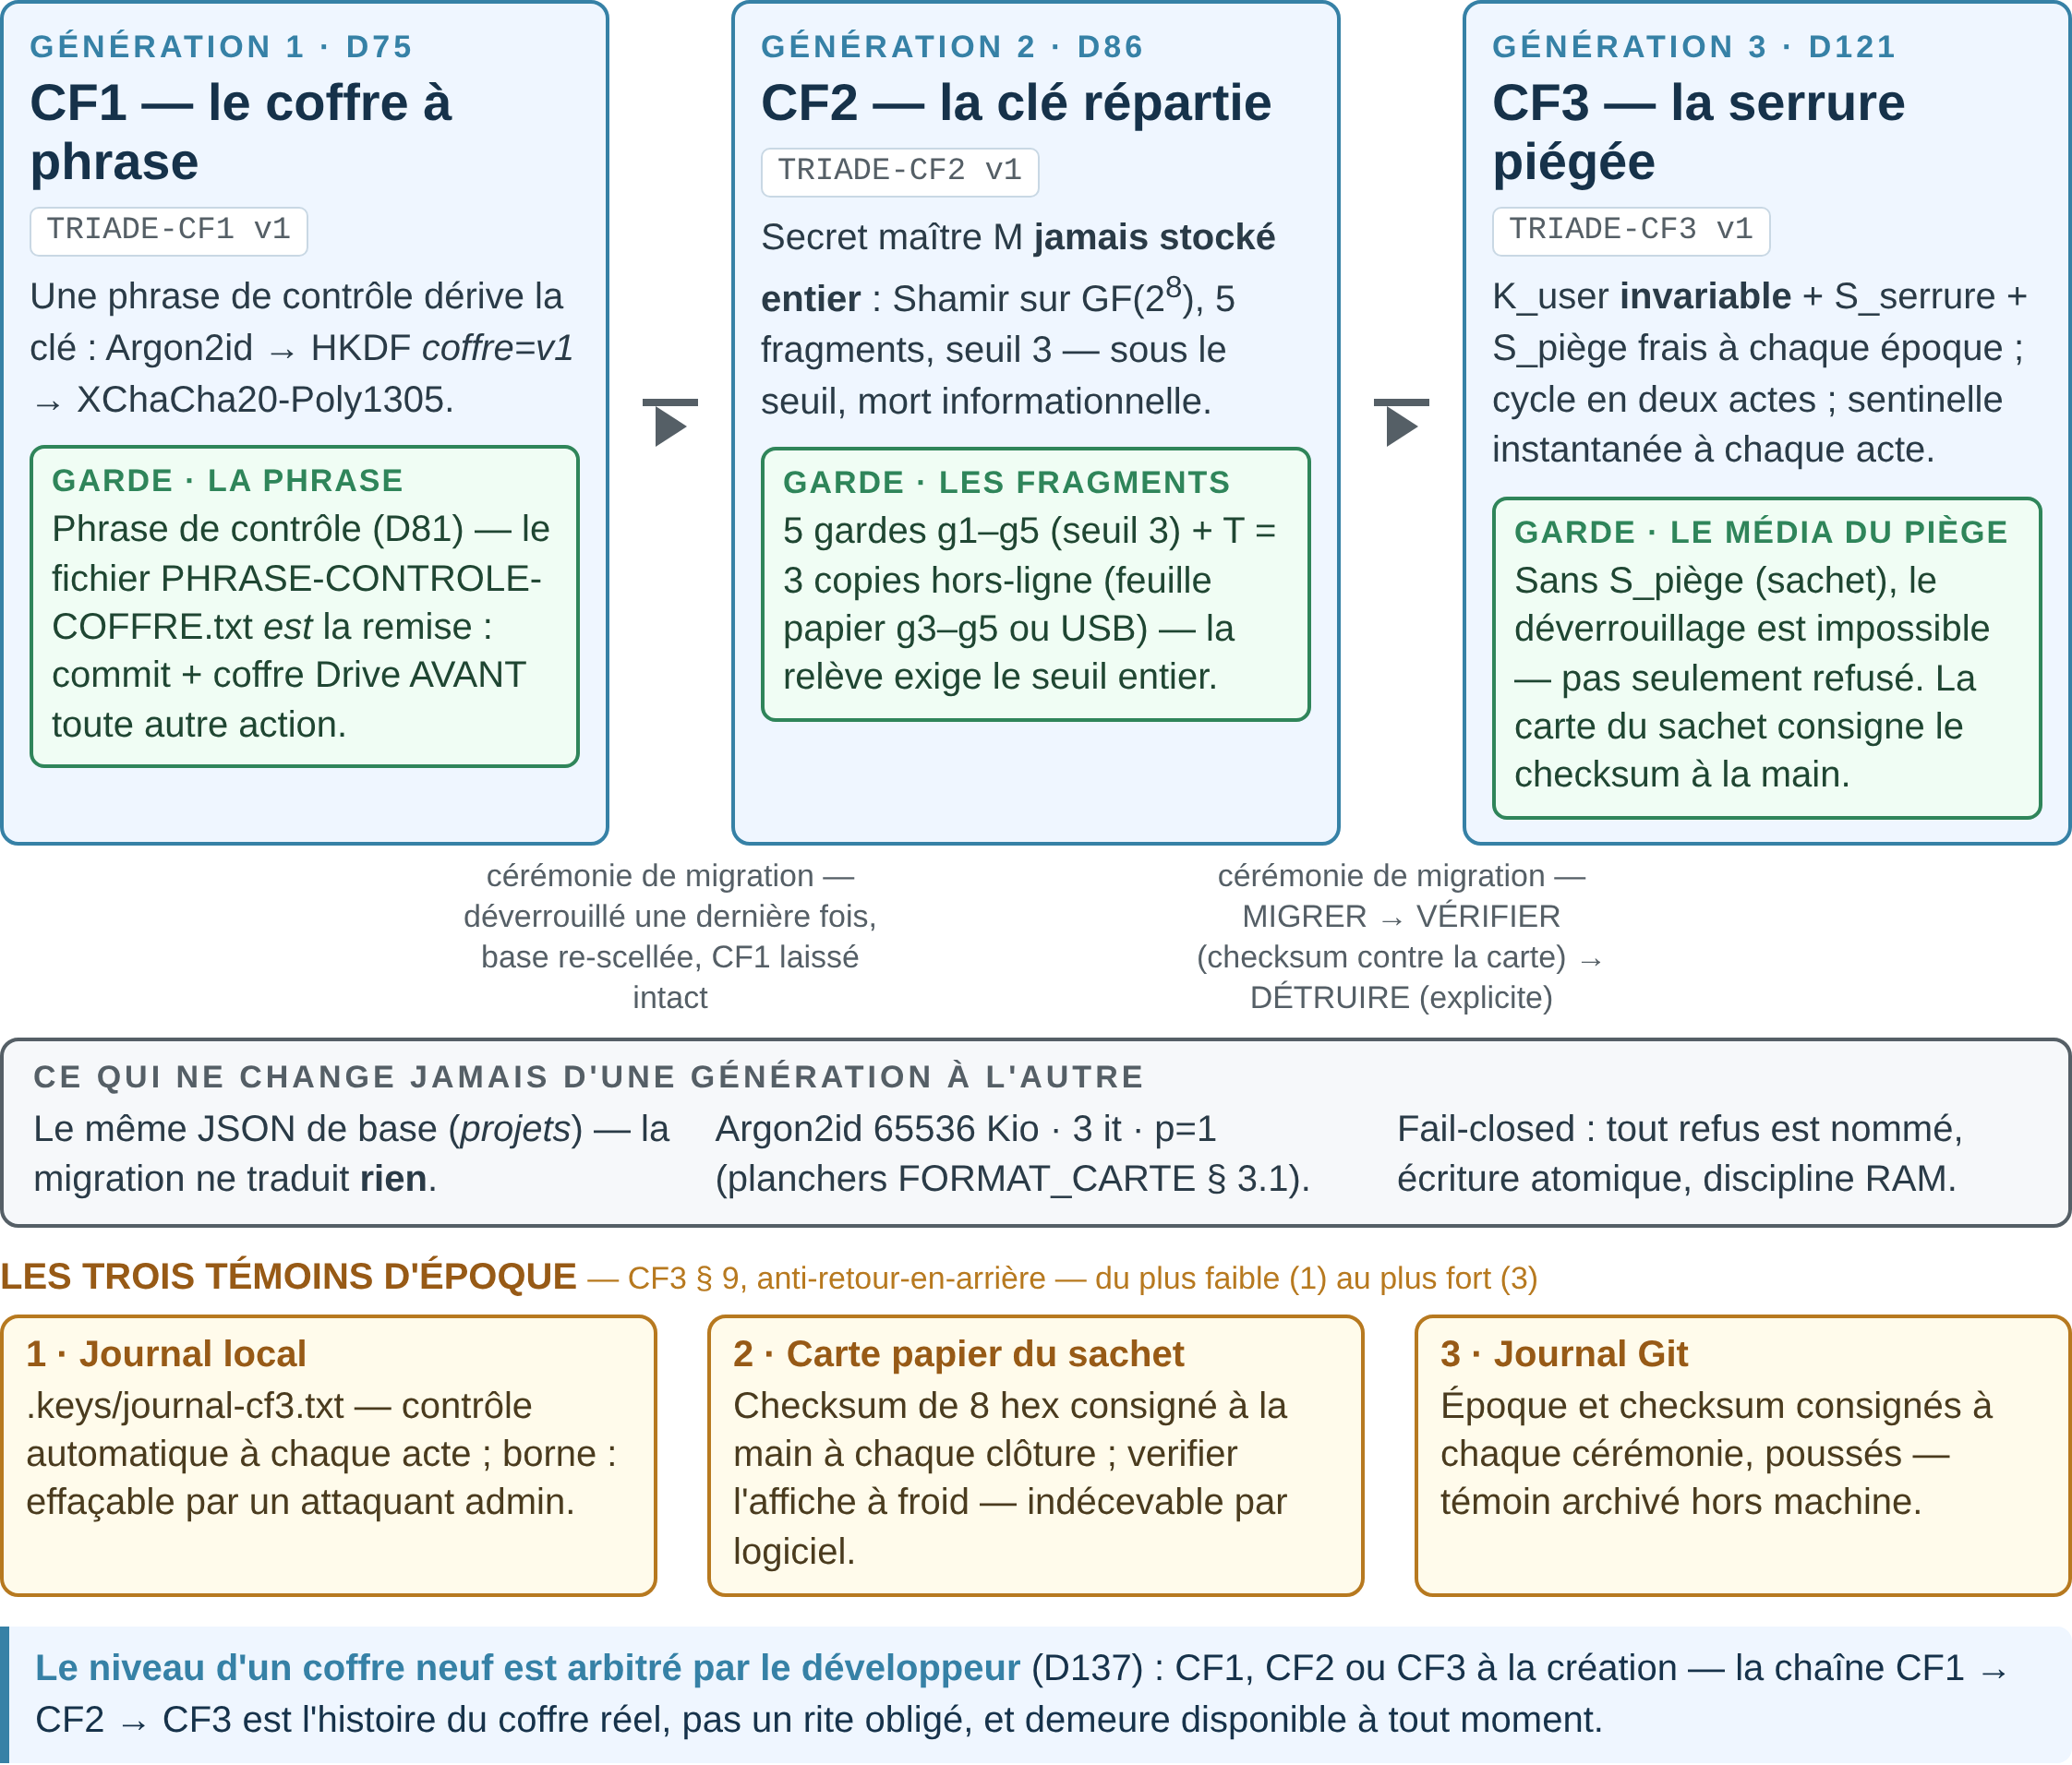
\includegraphics[width=\textwidth, max height=0.66\textheight]{chaine_cf}
\caption{La chaîne du coffre : trois générations, leurs gardes, les trois témoins
d'époque. Le niveau d'un coffre neuf est arbitré par le développeur (D137) — la
chaîne de migration est l'histoire du coffre réel, et demeure disponible à tout
moment.}
\label{fig:chaine}
\end{figure}

\subsection{Les trois générations, d'un coup d'œil}\label{sec:troisgenerations}

\begin{table}[htbp]
\centering\small
\caption{Les trois générations du coffre — d'un coup d'œil (le détail vit aux
chapitres 2 à 4).}
\label{tab:generations}
\begin{tabularx}{\textwidth}{@{}l Y Y Y@{}}
\toprule
 & \textbf{CF1} & \textbf{CF2} & \textbf{CF3} \\
\midrule
Née de & D75 (v0.5.1) & D86 (axe 2) & D121 (axe 4) \\
L'idée & une phrase suffit & la clé répartie vaut mieux & la serrure piégée
achève \\
Pour déverrouiller & la phrase & T fragments (seuil 3 sur 5) & la phrase ET le
piège d'époque égale \\
Ce qui peut manquer & la phrase (perdue = mort) & le seuil (sous 3 fragments =
mort informationnelle) & le média du piège (absent = acte impossible) \\
La garde vivante & la phrase sous séquestre 5/3 (amendé D223) & les gardes + la sentinelle & le sachet
+ la carte papier \\
Session & directe & directe, M effacé après l'acte & cycle en deux actes, brouillon
sous K\_session \\
Falsification prouvée & refus AEAD & refus AEAD + \code{verif} & destruction locale
+ PV — jamais le média \\
\bottomrule
\end{tabularx}
\end{table}

\subsection{Ce que le coffre N'EST PAS}\label{sec:pas}

Le coffre n'est pas un gestionnaire de mots de passe généraliste : il porte les
\emph{phrases maîtresses} du dépôt, pas vos comptes en ligne. Il n'est pas un coffre
d'artefacts : le dépôt git porte le code, la carte porte les empreintes — le coffre
porte ce qui \emph{ouvre} ces choses-là. Il n'est pas anonyme : chaque conteneur porte
son identité (magic, version, sel), chaque fragment son \code{coffre} (le sel, stable),
chaque piège son époque et son H\_projet. Et il n'est pas indulgent : une phrase
erronée est bénigne (réessai, délai croissant), mais une falsification \emph{prouvée}
détruit — la contrepartie qui rend le piège crédible (chapitre 4).

\subsection{Les trois règles du maître, avant tout le reste}\label{sec:troisregles}

\begin{enumerate}
\item \textbf{Jamais l'ancien avant le vert du neuf.} Chaque migration laisse l'ancien
conteneur intact jusqu'au verdict — CF1 est resté entier pendant la cérémonie CF2, CF2
est resté entier pendant la cérémonie CF3, et la destruction du CF2 reste un geste
explicite, après recoupement, sur machine froide de préférence.
\item \textbf{La phrase vit au séquestre, jamais au dépôt.} La garde active
est le séquestre D183 (D223) : cinq parts Shamir à seuil trois, les parts
inertes sous le seuil, la phrase en AUCUN dépôt — le dépôt est PUBLIC
(D220). La remise est la cérémonie de reconstitution à froid : trois parts
assemblées hors-ligne, la phrase reconstituée jamais écrite au dépôt,
l'usage transient détruit après le geste. Tout geste qui tenterait de
réécrire la phrase (ou son fichier) au dépôt est REFUSÉ avec son nom.
(La garde D81 — le fichier-remise commité — est l'histoire datée : la
phrase y demeure à vie, la rotation fut le remède ; cf. § \ref{sec:guarded81}.)
\item \textbf{Le sachet est individuel et il se garde comme un objet physique.} Un
média du piège par coffre ; les copies hors-ligne des fragments y vivent à côté des
pièges d'époque ; la carte papier y consigne les checksums à la main. Le sachet ne se
branche que pendant les actes qui l'exigent.
\end{enumerate}
   % Avant-propos · 1 Le coffre en une page
% =====================================================================
%  CH. 2 CF1 · CH. 3 CF2 · CH. 4 CF3 — LES TROIS GÉNÉRATIONS
% =====================================================================
\section{CF1 — le coffre à phrase (D75)}\label{sec:cf1}

\subsection{L'idée, et pourquoi elle a suffi un temps}

CF1 est né d'une demande du développeur : « stocker toutes les phrases maîtresses par
projet ». L'idée est la plus ancienne de la cryptographie symétrique : une phrase que
seul le maître connaît, dérivée en clé par une fonction coûteuse, protège tout le reste.
Elle a suffi un temps parce que la menace modélisée était simple — le \emph{vol au
repos} : un tiers qui s'empare du disque ou du dépôt ne doit rien pouvoir lire. Contre
cette menace, une phrase forte dérivée par Argon2id est une réponse complète.

Ce qui a fait grandir le coffre, c'est une autre menace, venue du terrain du
développeur : l'\emph{expropriation} (D84) — un tiers qui s'empare de la machine
\emph{pendant qu'elle vit}, phrase comprise. Contre elle, une phrase seule ne protège
pas : il faut que la clé n'existe nulle part entière. C'est l'histoire des deux
générations suivantes — CF1 n'est pas une erreur, c'est le socle : même CF3 dérive
K\_user par la même Argon2id aux mêmes planchers.

\subsection{La cérémonie de la clé}

\begin{lstlisting}
phrase (choisie par le maitre, D110 : alphanumerique, sans plafond)
  -> Argon2id(phrase, sel_argon 16 o, t=65536 Kio, m=3 it, p=1) = K_user 32 o
  -> HKDF-SHA256(K_user, sel_hkdf, info "coffre=v1") = KEK 32 o
  -> XChaCha20-Poly1305(JSON base, KEK, nonce 24 o frais, AAD = en-tete clair)
\end{lstlisting}

Le sel est propre au coffre (posé à l'init, 16 octets) ; le nonce est frais à
\emph{chaque écriture} ; l'empreinte du chiffretexte (sha256, posée dans l'en-tête)
nomme la corruption avant l'AEAD. La base claire est le JSON commun aux trois
générations :

\begin{lstlisting}
{ "format": ..., "protocole": ..., "cree": ..., "modifie": ...,
  "description": ..., "projets": { "<nom>": { "phrase": ..., ... }, ... } }
\end{lstlisting}

Chaque projet du dépôt y vit avec sa phrase maîtresse et ses métadonnées. Les gestes :
\code{init}, \code{lister}, \code{obtenir} (vers l'écran ou vers un fichier 0600),
\code{ajouter}, \code{retirer}, \code{verifier}, \code{changer-phrase},
\code{exporter}/\code{importer} (continuité), \code{bruler} (destruction manuelle).
L'autotest de falsification (19 contrôles à la naissance, D75) a établi la règle de la
maison : mauvaise phrase refusée ; mutation d'UN octet — chiffretexte, sel, nonce,
empreinte — chacune refusée nommément ; \code{lister} ne divulgue aucune phrase ;
l'export round-trip est exact.

\subsection{La garde de la phrase (D81) — le fichier fut la remise}\label{sec:guarded81}

L'épisode fondateur mérite d'être raconté, parce qu'il explique toute la discipline
actuelle. La rotation D80 avait produit une phrase neuve dont la remise — prévue « en
fin de tour » par affichage unique — n'a jamais eu lieu : la session d'exécution est
morte avant, d'une panne d'infrastructure de plus. La phrase ne vivait plus que dans le
bac à sable éphémère. Un décès d'infra de plus, et le coffre entier devenait
indéchiffrable à jamais. L'arbitrage est consigné : le risque de \textsc{perte} (vécu,
répété) dépasse le risque d'\textsc{exposition} (URL non devinable). De D81 au 19 novembre 2026 : dès sa
production — init, rotation, changement — la phrase était écrite dans
\code{PHRASE-CONTROLE-COFFRE.txt} (une ligne, rien d'autre), commitée au dépôt, poussée
(GitHub + miroir Drive par le hook) et posée au racine du coffre Drive, \emph{avant
toute autre action de la session}. Une phrase entrée dans l'histoire git y demeure à
vie : on ne compte plus sur sa confidentialité, la rotation reste le remède.
La garde plus dure EST VÉCUE depuis le 19 novembre 2026 (D223) : le
séquestre chiffré D183 — la phrase répartie en cinq parts à seuil trois
(cf. § \ref{sec:cerd183}) — la cérémonie VÉCUE, la garde ACTIVE est le
séquestre 5/3 ; la garde D81 est AMENDÉE (la phrase tournée, l'ancienne
demeurant ACTIVE jusqu'au geste vécu de sa destruction).

\section{CF2 — la clé répartie (D86)}\label{sec:cf2}

\subsection{L'idée : le secret qui n'existe nulle part}

CF2 répond à la question que CF1 laisse ouverte : que faire si l'adversaire tient la
machine \emph{vivante} ? La réponse de D86 : découper la clé maîtresse en fragments
tels qu'aucun supports ne suffise, et armer une sentinelle qui brûle les fragments si
un processus non autorisé lit la couche C. Le secret maître \textbf{M} (32 octets du
CSPRNG) n'est jamais écrit entier — nulle part, jamais : il vit reconstitué en RAM le
temps d'un déverrouillage, vérifié, puis effacé.

\subsection{Le découpage Shamir, en mots}

Un secret peut être \emph{réparti} : on le découpe en N fragments tels que n'importe
quels T d'entre eux le reconstituent, et que T$-1$ n'en disent \emph{rien} — pas
« difficile à calculer », \emph{rien} : la sécurité est informationnelle. Le mécanisme
(Shamir sur le champ GF($2^8$), polynôme générateur 0x11B — celui d'AES) : pour chacun
des 32 octets de M, un polynôme distinct de degré $T-1$ dont les coefficients sont
frais du CSPRNG ; le fragment $j$ porte les évaluations de ces polynômes au point
$x_j$. T fragments régressent les polynômes (Lagrange en $x=0$) et retrouvent M ;
T$-1$ fragments laissent tout M' possible — aucune discrimination, aucune attaque.

L'arbitrage terrain : \textbf{N = 5, T = 3}. Cinq gardes machine (répertoires distincts,
un fragment chacun, mode 0700) ; la relève exige \textbf{T copies hors-ligne} — trois
à seuil 3 : deux copies laisseraient le coffre mort si les gardes machine brûlaient
(l'autotest le prouve par restauration partielle refusée). Brûler les cinq gardes
machine = mort du coffre ; le code volé reste inexploitable (les enveloppes de carte
sont mortes avec lui) ; restaurer trois copies hors-ligne = résurrection. C'est un
contrat clair : \emph{ce que vous acceptez de perdre} contre \emph{ce que vous refusez
de voir exfiltré}.

\subsection{Les fragments — le format qui se transporte sur papier}

\begin{lstlisting}
TRIADE-CF2-FRAG v1
coffre: <sel HKDF du conteneur, 64 hex - l'identite STABLE du coffre>
x: <indice, decimal>
seuil: t=3/n=5
fragment: <64 hex - 32 o>
tag: <16 hex - sha256("TRIADE-CF2-frag" || x || fragment) tronque>
\end{lstlisting}

Le fragment est ASCII autodescriptif : il se lit, s'imprime, se recopie — l'exfiltration
d'un fragment est un vol physique, hors du modèle. Il est lié au \emph{sel} du coffre
(l'identité stable, posée à l'init) et jamais à l'empreinte de l'en-tête (le nonce
change à chaque écriture ; une liaison à l'en-tête invaliderait les copies papier à
chaque mutation — la faute a été dénoncée par le parcours CLI complet avant d'être
commise, D106). Le \code{tag} nomme le fragment fautif sans le divulguer : corruption,
mélange de fragments d'un autre coffre (sel divergent), collision d'indice — refus
nommés à l'import comme à la reconstitution.

\begin{terrain}[— les cinq originaux, la feuille et les copies (D131)]
La question du terrain, 31/10 : « la cérémonie m'a produit un fragments-cf2.txt et le
système attend 3 fragment-*.cf2 ». Les CINQ originaux vivent sous
\code{.keys\textbackslash gardes-cf2\textbackslash g1...g5\textbackslash
fragment-N.cf2f} — un fichier par garde, dans un dossier caché du clone. La FEUILLE
est l'export papier des TROIS fragments g3--g5 (les tags sont vérifiés avant
impression) : c'est une empreinte humaine, à ranger au sachet. Les COPIES USB sont les
fichiers \code{.cf2f} eux-mêmes, copiés hors-ligne : c'est eux que le contrôle de
relecture relit. La feuille et les copies ne sont pas le même objet — l'un se recopie
à la main, l'autre se restaure.
\end{terrain}

\subsection{Le conteneur, la sentinelle, la porte}

Le conteneur \code{TRIADE-CF2} dérive sa clé de M (HKDF, contexte \code{coffre=v2} —
nul chevauchement avec CF1 ni avec les fragments de carte) ; le champ \code{verif}
(16 octets) vérifie toute reconstitution avant que l'AEAD ne parle. La
\textbf{sentinelle} surveille la couche C (jamais les gardes ni le conteneur) à
\emph{double seuil} : un processus hors liste blanche \emph{et} une lecture de
contenu — deux signaux indépendants, parce qu'une fausse alerte serait une perte
auto-infligée. Moteur laboratoire : inotify + attribution \code{/proc} ; moteur de
production Windows : SACL + journal 4663 ou ETW (exigence consignée). La
\textbf{PORTE D120} — née de la demande du terrain : « si le déverrouillage est tenté
et qu'elle n'est pas lancée, tous nos efforts sont inutiles » — exige une sentinelle
vivante pour déverrouiller ; sur plateforme sans moteur, la porte \emph{avertit
nommément} à chaque déverrouillage. Le chapitre 5 raconte la fin de cette histoire.

La \textbf{liste blanche} de la sentinelle mérite son mot : elle blanchit par motifs
regex sur l'image de processus résolue \emph{et} sur la ligne de commande complète —
jamais « tout python3 » : c'est la ligne qui distingue \code{build\_m4.py} d'un
\code{-c} jetable. La liste est MINIMALE par construction (chaînes de build,
vérificateurs, l'éditeur du maître, la sentinelle elle-même) et testée par
falsifiabilité : un motif trop large blanchirait l'adversaire — c'est le défaut que
la suite prouve ne pas avoir.

La \textbf{destruction} (\code{bruler}) : trois passes d'écrasement (aléa, 0xFF, 0x00),
troncature, renommage aléatoire, unlink, fsync — et un \textbf{procès-verbal} nommant
le déclencheur (pid, image, fichier lu). Le conteneur et les gardes vides restent sur
place : le PV dit la mort, la vérification la confirme. La \textbf{restauration}
(\code{restaurer}) est atomique : chaque fragment est vérifié (tag + sel + indice
libre) et toute anomalie laisse \emph{rien} s'écrire — une remise partielle serait un
coffre menteur.

\subsection{Les critères de sortie de CF2 — et leurs preuves}

La spec scellée lie chaque promesse D86 à une preuve mesurable
(\code{v06/test\_cf2.py}) ; le maître peut les re-voir à volonté :

\begin{table}[htbp]
\centering\small
\caption{Critères de sortie D86 et leurs preuves (CF2).}
\label{tab:sortiecf2}
\begin{tabularx}{\textwidth}{@{}Y Y@{}}
\toprule
\textbf{Critère D86} & \textbf{Preuve} \\
\midrule
Shamir : reconstitution, seuil, refus nommés & T1 — KAT + 1000 vecteurs, interop
exhaustive C(5,3) \\
Sous T : informationnellement mort & T2 — un M' arbitraire accepté par les fragments
seuls : aucune discrimination \\
Conteneur : round-trip + fail-closed & T3 — en-tête, AEAD, \code{verif}, empreinte :
refus nommés \\
Exfiltration simulée $\to$ fragments détruits, indéchiffrable & F1 — sentinelle en
sous-processus, lecture non blanchie, PV + mort du coffre, restauration $\to$ vie : le
cycle complet \\
Fausses alertes NULLES en essai nominal & T4 — opérations blanches (build,
vérificateur simulés) : journal « blanchi », zéro brûlage \\
Latence détection $\to$ destruction bornée & F1 — mesurée, assertée sous la borne
consignée \\
Remise douteuse refusée sans écrire & F2 — atomicité, octet pour octet \\
Santé de la sentinelle & T5 — heart-beat frais, mort visible \\
\bottomrule
\end{tabularx}
\end{table}

\section{CF3 — la serrure piégée (D121)}\label{sec:cf3}

\subsection{L'idée : le témoin qui ne peut pas mentir}

CF3 est né de deux demandes du terrain, servies ensemble : « plutôt qu'une sentinelle
externe, une serrure du coffre piégée » et « une vulnérabilité réside durant le temps
où la session est ouverte ». L'idée : couper la clé en trois éléments dont l'un vit
\emph{hors machine} — le piège. Sans lui, le déverrouillage n'est pas refusé, il est
\emph{impossible} : il manque une moitié de la serrure. Et comme le piège est hors
machine, aucun état de machine falsifiable ne peut le remplacer : c'est un témoin que
le logiciel ne peut ni imiter ni truquer.

\subsection{Les trois éléments et l'époque}

\begin{itemize}
\item \textbf{K\_user} — la clé de l'utilisateur, \code{Argon2id(phrase,
sel\_argon)} : \emph{invariable à travers les époques} (la demande du terrain : « clé
utilisateur qui ne change pas »). Le sel et les paramètres sont posés à l'init et
jamais retouchés.
\item \textbf{S\_serrure} — la moitié « serrure » : 32 octets frais du CSPRNG à
\emph{chaque époque}, logée dans l'en-tête clair du conteneur (côté machine).
\item \textbf{S\_piège} — la moitié « piège » : 32 octets frais à chaque époque,
logée \emph{exclusivement sur le média séparé} — jamais écrite sur la machine hors
l'instant de l'acte.
\end{itemize}

L'\textbf{époque} (u64, posée à 1, incrémentée à chaque clôture) est l'horloge de la
métamorphose : chaque clôture renouvelle les moitiés, si bien qu'un secret volé ne
sert qu'une époque. \textbf{H\_projet} (sha256 de l'état scellé) lie la clé de clôture
au contenu — la course de clôture, § \ref{sec:course}.

\subsection{La dérivation et le champ qui ferme l'essai-hors-ligne}

\begin{lstlisting}
KEK = HKDF-SHA256(ikm = K_user || S_serrure || S_piege ;
                  salt = sel_hkdf ;
                  info = "triade-CF3/v1|" || epoque(le64) || H_projet)
verif = sha256(HKDF(ikm = K_user || V_piege ;
                    info = "triade-CF3/verif/v1"))[:16]
chiffretexte = XChaCha20-Poly1305(clair, KEK, nonce 24 o,
                                  AAD = en-tete jusqu'au nonce, 168 o)
\end{lstlisting}

Le champ \code{verif} est subtil et il mérite une phrase : le voleur de la
\emph{machine seule} ne peut même pas \emph{tester} des phrases contre le conteneur —
il lui manque V\_piège, la valeur publique qui vit sur le média. Le brute-force
hors-ligne n'est pas difficile, il est \emph{sans objet}. Contre le voleur de tout
(machine + média), la défense est Argon2id — borne consignée, même famille que CF1.

\subsection{Le fichier piège — un ASCII par époque}

\begin{lstlisting}
TRIADE-CF3-PIEGE v1
epoque: <u64 decimal>
projet: <H_projet hex (64)>
piege: <S_piege hex (64)>
verif: <V_piege hex (32)>
tag: <hex (16)>
\end{lstlisting}

Un fichier par époque, sur le média du sachet : \code{piege-CF3-epoque-1.txt},
\code{-2.txt}, \ldots{} Une clôture \textbf{ajoute} le piège N+1 et ne ronge jamais
les pièges passés — l'ancien piège est la relève du canonique précédent (si le média
perd le dernier piège, l'avant-dernier ne résurrect rien, mais il témoigne). Le
\code{tag} nomme la corruption du média sans divulguer ; un piège entièrement forgé se
présente comme une phrase erronée — bénin, refus nommé, jamais de destruction. Demain,
le média pourra être une clé USB à bouton physique (FIDO2) : seul le support change.

\subsection{Le cycle en deux actes — la fenêtre de session bornée}\label{sec:deuxactes}

\begin{enumerate}
\item \textbf{Acte I — ouverture.} Phrase + piège branché $\to$ sentinelle
instantanée (§ \ref{sec:sentinst}) $\to$ clair $\to$ \emph{brouillon} chiffré sur
disque sous une clé de session éphémère K\_session, qui ne vit qu'en RAM dans l'objet
Session. Puis K\_user, KEK et les moitiés sont effacés ; le média du piège est
\textbf{débranché} — geste humain, consigné au journal de cérémonie ; le conteneur
canonique n'est \emph{jamais} réécrit pendant la session.
\item \textbf{Session.} Lecture et écriture sur le brouillon (AEAD sous K\_session).
Une panne ou un abandon tue K\_session avec le processus : le brouillon devient un
déchet indéchiffrable, le canonique reste scellé. \emph{Une panne auto-nettoie.}
\item \textbf{Acte II — clôture.} Média rebranché, phrase \textbf{retapée} (une faute
de frappe est bénigne — aucun scellement n'a lieu). H\_final = sha256 du brouillon
final, checksum court de 8 hex \emph{affiché} : l'humain recoupe avec sa carte. Moitiés
fraîches, époque N+1, KEK de clôture dérivé \emph{avec} H\_final. Écriture du piège
N+1 (additive) puis du conteneur en \emph{staging} ; \textbf{re-lecture à froid} du
staging par la sentinelle complète — verte : remplacement atomique ; échec : staging
détruit, canonique et brouillon intacts, la clôture est rejouable.
\end{enumerate}

\subsection{La course de clôture et l'étiquette}\label{sec:course}

L'attaque : un malware attend la frappe de phrase à la clôture, vole la clé dérivée et
scelle \emph{son} état à la place. La parade est double. D'abord, la clé de clôture
est dérivée \emph{avec} H\_final : elle ne peut sceller que l'état exact dont le hash a
servi à la dériver. Ensuite, l'\textbf{étiquette} est vérifiée à l'ouverture : le clair
déchiffré doit hacher vers le H\_projet de l'en-tête. Le faux conteneur « étiquette
honnête, contenu substitué » est démasqué : sha256(contenu) $\neq$ H\_projet —
falsification \emph{prouvée}, destruction locale. Un KEK volé ne produit donc aucun
conteneur ouvrable pour un autre contenu, et le faux conteneur exige en outre d'écrire
le média du piège pendant qu'il est branché.

\subsection{Les trois témoins d'époque}\label{sec:temoins}

Le roll-back restaure un \emph{couple} cohérent (conteneur N + piège N) — l'AEAD
passerait seul. La défense est graduée : le \textbf{journal local}
(\code{.keys/journal-cf3.txt}) contrôle automatiquement à chaque acte (époque du
conteneur $\geq$ époque du miroir, sinon « RETOUR EN ARRIÈRE » nommé) mais un attaquant
admin peut l'effacer ; la \textbf{carte papier du sachet} consigne le checksum de 8 hex
à la main à chaque clôture — indécevable par logiciel ; le \textbf{journal Git}
(consigné à chaque cérémonie de clôture, poussé) est le témoin archivé hors machine.
Le verdict à froid (\code{verifier}) affiche le checksum pour le recoupement humain :
\emph{la machine dit, la carte confirme, vous seul jugez}.

\begin{terrain}[— ce que dit un verdict réel]
Extrait du rapport de migration du coffre réel (30/10/2026, boîte noire du GUI) — le
format que vous verrez à chaque \code{verifier} :
\begin{lstlisting}
[CF3] VERDICT : VERT - epoque 1, checksum 0cc89a96
    (carte papier / journal Git : recoupez), 1 projet(s)
\end{lstlisting}
Époque, checksum, projet(s) : les trois choses à recouper. Le checksum se note sur la
carte du sachet, l'époque se suit d'une clôture à l'autre, le compte de projets doit
être le vôtre.
\end{terrain}

\subsection{Les critères de sortie de CF3 — et leurs preuves}

Même loi (\code{v06/test\_coffre\_cf3.py}, la suite de falsifiabilité) :

\begin{table}[htbp]
\centering\small
\caption{Critères de sortie CF3 et leurs preuves.}
\label{tab:sortiecf3}
\begin{tabularx}{\textwidth}{@{}Y Y@{}}
\toprule
\textbf{Critère} & \textbf{Preuve attendue} \\
\midrule
Round-trip deux actes & init $\to$ ouvrir $\to$ modifier $\to$ fermer $\to$ ouvrir :
contenu exact, époque incrémentée, moitiés remplacées, \code{sel\_argon} invariant \\
Phrase erronée (acte I ET II) & refus nommé, JAMAIS de destruction, aucune écriture \\
Piège absent & déverrouillage impossible, refus nommé \\
Piège périmé / roll-back du couple & refus nommé + journal \\
Tag du piège invalide & refus nommé SANS destruction (média hors limite) \\
Falsification prouvée côté machine & destruction locale + PV nommé, média et fragments
intacts \\
Course de clôture & KEK volé + faux conteneur (étiquette menteuse OU honnête à
contenu substitué) : refus + destruction, jamais une ouverture \\
Panne simulée à chaque phase de clôture & canonique intact, cycle rejouable \\
Auto-nettoyage par panne & brouillon indéchiffrable sans K\_session, canonique jamais
réécrit pendant la session \\
Non-régression & sceau\_I verifier CODE 0, suites CF2/sceau-I/GUI vertes \\
\bottomrule
\end{tabularx}
\end{table}
   % 2 CF1 · 3 CF2 · 4 CF3
% =====================================================================
%  CH. 5 LA SENTINELLE · CH. 6 LES SECRETS ET LEURS GARDES
% =====================================================================
\section{La sentinelle — du démon à la serrure}\label{sec:sentinelle}

\subsection{Pourquoi ce mot revient, et ce qu'il a voulu dire trois fois}

« Sentinelle » a désigné trois choses différentes dans l'histoire du coffre, et la
confusion des trois est la question la plus fréquente du terrain. Une fois pour
toutes :

\begin{table}[htbp]
\centering\small
\caption{Les trois vies du mot « sentinelle ».}
\label{tab:sentinelles}
\begin{tabularx}{\textwidth}{@{}l Y Y@{}}
\toprule
\textbf{Époque} & \textbf{Ce que c'était} & \textbf{Sa limite} \\
\midrule
CF2, démon résident (D86) & un processus userland de longue durée : surveille la
couche C, croise deux seuils (processus non blanchi + lecture de contenu), brûle les
fragments & usurpable par un faux heart-beat ; tuable par l'adversaire avant
destruction ; exige un moteur de plateforme (inotify/\code{/proc} au laboratoire,
SACL/ETW attendus sur Windows) \\
CF2, PORTE D120 & le verrou qui refuse de déverrouiller sans sentinelle vivante — la
demande du terrain : « si elle n'est pas lancée, tous nos efforts sont inutiles » &
sur plateforme sans moteur, la porte \emph{avertit} à chaque déverrouillage (« SANS
sentinelle ») : l'ère intermédiaire est honnête mais incomplète \\
CF3, sentinelle instantanée (D121) & \textbf{par invocation} : les cinq vérifications
ordonnées courent DANS chaque acte qui déverrouille — ouvrir, clôture,
\code{verifier}, re-lecture à froid & aucune : elle ne dépend d'aucun état de machine
falsifiable — \emph{le piège est le témoin, et il est hors machine} \\
\bottomrule
\end{tabularx}
\end{table}

La question du terrain, posée à la passation : \emph{« on avait pas décidé de la
supprimer, en migrant en CF3 ? Si on impose CF3 dès la création de projet, on n'a pas
besoin de sentinelle, non ? »} La réponse tient en trois temps. Oui, le \textbf{démon}
est mort en CF3 — remplacé, pas retiré. L'exigence D120 (« indispensable au
déverrouillage ») \emph{reste}, réalisée par invocation : la sentinelle instantanée
n'est pas un composant qu'on peut oublier de lancer, \emph{c'est la serrure elle-même}
— le sine qua non est satisfait par construction, sans démon ni moteur de plateforme à
attendre. Et oui, \textbf{un coffre né CF3 n'a jamais connu de sentinelle à lancer} :
\code{init} le crée à l'époque 1 avec son média du piège, et chaque acte porte sa
propre vérification.

\subsection{La sentinelle instantanée — l'ordre est la loi}\label{sec:sentinst}

À tout acte qui déverrouille, cinq vérifications courent \emph{dans cet ordre} —
l'ordre n'est pas esthétique, il sépare les modes de défaillance :

\begin{enumerate}
\item \textbf{Piège présent.} Absent : refus nommé, déverrouillage \emph{impossible}
(fail-closed). Rien n'est lu, rien ne brûle — l'absence du média n'est jamais une
attaque, c'est un état.
\item \textbf{Piège intègre} (le \code{tag}). Invalide : refus nommé + journal, mais
\emph{pas} de destruction — le média est hors limite de confiance : une corruption
bénigne (lecteur capricieux, secteur mort) doit pouvoir être relue depuis les copies
hors-ligne. La destruction attend la preuve cryptographique (étape 5).
\item \textbf{Cohérence des champs publics.} Époque du piège = époque du conteneur
(sinon : « piège PÉRIMÉ », refus anti-retour) ; H\_projet du piège = H\_projet du
conteneur (sinon : le piège d'un \emph{autre} coffre).
\item \textbf{Phrase} (via \code{verif}). Divergente : réessai à délai croissant —
1, 2, 4 secondes, plafond 8 (le plafond borne aussi le verrouillage de compte par
soi-même). \emph{Jamais} de destruction : une faute de frappe ne doit pas tuer le
coffre.
\item \textbf{AEAD + étiquette} (KEK complet). Échec \emph{après} 1--4 verts :
falsification ou corruption \emph{prouvée} côté machine $\to$ destruction locale +
PV + journal. L'étiquette vérifiée (le clair doit hacher vers le H\_projet de
l'en-tête) ferme la course de clôture.
\end{enumerate}

Un échec \textbf{nomme son étape} ; les étapes suivantes ne courent pas. C'est la
grammaire même du fail-closed : vous saurez toujours \emph{quoi} a refusé, et donc
\emph{où} regarder (chapitre 9).

\begin{terrain}[— l'avertissement D120 dans un rapport réel]
Pendant la migration du coffre réel (30/10), le \emph{déverrouillage CF2} — la
dernière fois que la vieille serrure parlait — a affiché :
\begin{lstlisting}
[coffre-CF2] AVERTISSEMENT D120 : deverrouillage SANS
sentinelle vivante - le moteur n'est pas livre sur cette
plateforme (exigence consignee spec  9) : le coffre s'ouvre
sans temoin.
\end{lstlisting}
Aucun avertissement équivalent n'est apparu aux actes CF3 : la sentinelle instantanée
n'a pas de moteur à attendre. L'avertissement D120 est le signal d'une \emph{ère} —
honnête, bornée, et close par la génération suivante.
\end{terrain}

\subsection{Ce que la destruction locale ne touche JAMAIS}

La réponse à la falsification (étape 5) détruit \emph{côté machine} : le conteneur, le
staging, le brouillon — trois passes d'écrasement (aléa, 0xFF, 0x00), troncature,
renommage aléatoire, unlink, fsync, et un PV horodaté dans \code{.keys/pv-cf3/} avec la
raison nommée (deux destructions la même seconde produisent deux fichiers distincts —
correctif D123, appris d'un écrasement prouvé par le terrain). Elle ne touche
\textbf{jamais} le média du piège (c'est la relève), \textbf{jamais} les fragments CF2
ni leurs copies hors-ligne : la destruction reste survivable — c'est la contrepartie
qui rend le piège destructif acceptable. La mort d'un coffre est toujours un état
\emph{recouvrable par le sachet}.

\section{Les secrets et leurs gardes}\label{sec:gards}

\subsection{L'inventaire honnête — ce que vous protégez, en fait}

\begin{table}[htbp]
\centering\small
\caption{Les secrets du coffre et leurs gardes — l'inventaire complet.}
\label{tab:inventaire}
\begin{tabularx}{\textwidth}{@{}l Y Y@{}}
\toprule
\textbf{Secret} & \textbf{Sa garde} & \textbf{Si la garde manque} \\
\midrule
La phrase de contrôle & votre tête ; le séquestre D183/D223 (cinq parts
Shamir à seuil trois, la reconstitution à froid) & sans la phrase, pas de
K\_user — le coffre est muet ; sous trois parts assemblables, la phrase est
PERDUE (le seuil est la survie) \\
Les phrases par projet & le coffre chiffré (CF1/2/3) & un projet dont la phrase est
perdue doit faire l'objet d'une rotation de sa propre lignée \\
Le secret maître M (CF2) & cinq fragments Shamir, seuil 3 — jamais entier nulle part &
sous 3 fragments : mort \emph{informationnelle} (aucune attaque possible, aucune
reconstruction non plus) \\
S\_piège (CF3, par époque) & le média du sachet — jamais sur la machine hors l'instant
de l'acte & sans le piège d'époque égale : l'acte est \emph{impossible} — branchez le
bon média \\
La graine de clé I & support physique hors-ligne (64 hex — imprimable) & le dépôt
porte la clé publique ; une graine perdue attend la rotation de clé (re-signer tous
les arbres, même commit) \\
\bottomrule
\end{tabularx}
\end{table}

\subsection{Le sachet — l'objet physique qui vaut le coffre}

Le sachet est une pochette physique, \textbf{individuelle} (un média du piège par
coffre — borne consignée), qui porte : les \textbf{pièges d'époque}
(\code{piege-CF3-epoque-N.txt}, un fichier par époque, ajoutés à chaque clôture) ; les
\textbf{copies hors-ligne des fragments CF2} (T = 3 : la relève si les gardes machine
brûlent) ; et la \textbf{carte papier}. Il se branche pendant les actes qui l'exigent —
et \emph{seulement} pendant eux : le geste de débrancher est consigné au journal de
cérémonie, parce qu'un média resté branché pendant la session est un média exposé.

\subsection{La carte du sachet — le témoin indécevable}

La carte est une fiche papier, écrite \emph{à la main}, une ligne par clôture :

\begin{lstlisting}
TRIADE - coffre CF3 (carte du sachet)
2026-10-30  epoque 1   checksum 0cc89a96
                                (migration CF2 -> CF3, VERIFIER VERT x2)
<ligne suivante a la prochaine cloture - jamais d'effacement>
\end{lstlisting}

Sa raison d'être : l'anti-retour-en-arrière (§ \ref{sec:temoins}). Un attaquant admin
peut effacer le journal local et vous resservir un conteneur ancien avec son piège
ancien — il ne peut pas imiter votre écriture dans votre sachet. Le jour où
\code{verifier} affiche un checksum absent de votre carte, le mensonge est nommé.
La carte ne protège que si elle est \emph{regardée} : le verdict à froid ré-exécuté
par la machine est le filet (recommandation : machine froide, le lendemain d'une
cérémonie).

\subsection{La frontière des supports — git, \code{.keys}, sachet, Drive}

\begin{table}[htbp]
\centering\small
\caption{La frontière des supports — ce qui vit où, et pourquoi.}
\label{tab:frontiere}
\begin{tabularx}{\textwidth}{@{}l Y Y@{}}
\toprule
\textbf{Support} & \textbf{Ce qu'il porte} & \textbf{Ce qu'il ne porte JAMAIS} \\
\midrule
Dépôt git (poussé, PUBLIC depuis D220) & le code, la spécification signée
(\code{v06/I/}), les preuves publiques du sceau, le journal de travail & aucun
conteneur, aucun fragment, aucune graine, AUCUNE PHRASE (le séquestre 5/3
hors dépôt, D223) : \code{/.keys/} est gitignoré \\
\code{.keys/} du clone & conteneurs CF1/CF2/CF3, gardes CF2, config, journaux et PV
locaux, miroir d'époque & jamais dans git — la ligne existe depuis D12/D27, le
coffre-fort depuis D75 \\
Le sachet & pièges d'époque, T copies hors-ligne, la carte papier & jamais branché
pendant une session de travail \\
Le Drive & le miroir complet du dépôt, le kit de cérémonie (\code{v06/} identique au
miroir par construction, D130), le conteneur CF1 de secours & aucune graine de clé I \\
\bottomrule
\end{tabularx}
\end{table}

\begin{terrain}[— rien à pousser après une cérémonie de coffre]
La question du terrain, juste après la migration CF3 : « je dois pousser quelque chose
sur le git maintenant ? » Non — par construction. Tout ce que la migration écrit vit
dans \code{.keys\textbackslash} (ignoré : ligne 28 du \code{.gitignore}), le piège vit
sur le média, la boîte noire est un \code{*.log} (ignoré). Un \code{git status} rend
\code{nothing to commit} : le clone est exactement ce que GitHub a. Les seuls
\emph{push} de votre chaîne sont les remises du sceau — et ceux-là, la cérémonie du
sceau les guide. La consignation au \emph{journal Git} (le troisième témoin d'époque)
se fait côté laboratoire, par le commit qui accompagne le rapport D122.
\end{terrain}

\subsection{La rotation — le remède quand un secret a pu fuir}\label{sec:rotation}

La phrase commise en git y demeure à vie (D81) ; le média photographié pendant un acte
sert une époque (borne assumée). Le remède n'est jamais d'espérer : c'est de
\emph{tourner}.

\begin{table}[htbp]
\centering\small
\caption{Les rotations du coffre — quoi tourne, quand, et ce qui ne change pas.}
\label{tab:rotations}
\begin{tabularx}{\textwidth}{@{}l Y Y@{}}
\toprule
\textbf{Rotation} & \textbf{Le geste} & \textbf{Ce qui ne change pas} \\
\midrule
Phrase de contrôle & \code{changer-phrase} (l'ancienne devient inopérante, les
entrées intactes) ; le changement passe par la cérémonie sous séquestre —
trois parts assemblées à froid, la phrase neuve re-découpée en CINQ parts,
JAMAIS écrite au dépôt (le refus nommé la garde) & le coffre, les projets,
le sel (le re-chiffrement prend un sel neuf) \\
Moitiés CF3 & chaque \emph{clôture} : S\_serrure et S\_piège frais, époque N+1 &
K\_user, \code{sel\_argon} — la clé utilisateur est INVARIABLE à travers les
époques \\
Secret maître CF2 & re-découpage Shamir (rotation complète du coffre CF2) & la base
JSON, le seuil \\
Clé I du sceau & remplacer \code{cle-publique-I.txt} ET toutes les signatures dans le
MÊME commit (un état mixte est refusé par \code{verifier}) ; la rotation est consignée
au journal & les arbres, les manifestes (re-signés par la nouvelle clé) \\
\bottomrule
\end{tabularx}
\end{table}

La règle de jugement : une exposition \emph{prouvée} (phrase vue, média photographié)
exige la rotation dans la session qui suit ; une exposition \emph{possible} (doute,
reliquat) se traite au calendrier. Entre les deux, votre degré de sommeil est le
dernier arbitre — c'est à vous que la menace s'adresse.
   % 5 La sentinelle · 6 Les secrets et leurs gardes
% =====================================================================
%  CH. 7 LES CÉRÉMONIES · CH. 8 LE RUNBOOK DU MAÎTRE
% =====================================================================
\section{Les cérémonies — le maître fait, l'outil relaie}\label{sec:ceremonies}

\subsection{Le principe : personne ne touche vos secrets à votre place}

Toutes les cérémonies du coffre obéissent à la même discipline (D105) : le bac à
sable — l'agent, l'assistant, whatever — ne touchera \emph{jamais} le conteneur ni
les phrases réels. Les cérémonies sont des actes du maître, guidés par un outillage
qui \emph{relaie} sans réimplémenter : le GUI lance les vérités vivantes
(\code{coffre\_cf2.py}, \code{coffre\_cf3.py}, \code{sceau\_I.py}) et leur sortie
coule à l'écran. La phrase passe par STDIN — jamais en ligne de commande (invisible
des journaux de processus), jamais affichée, jamais dans un rapport. Le verdict est
\textbf{croisé} : code de sortie \emph{et} marque attendue dans le flux — un enfant
menteux qui affiche VERT mais sort 1 est ROUGE ; un enfant muet est SANS VERDICT.

Chaque module à tester porte le \textbf{trio D122} : une GUI, une boîte noire locale
(journal horodaté, gitignoré, muet si le disque refuse — témoin, pas dépendance), un
bouton « Envoyer le rapport ». Le rapport emporte l'écran et la boîte noire, aucune
phrase, aucun chemin de coffre réel.

\subsection{La cérémonie du sceau de l'Intention (quatre gestes)}\label{sec:cersceau}

Le sceau signe la spécification elle-même — l'arbre \code{v06/I/} et les treize
arbres de lignée : le garde est à QUATORZE arbres signés (D177 — l'arbre
\code{loupe} entré à la table canonique par la cérémonie d'ère du TGN).
Quatre gestes, depuis le clone :

\begin{enumerate}
\item \textbf{Préparer} (le dépôt) : \code{sceau\_I.py preparer} reconstruit le
manifeste de chaque arbre, compare au manifeste signé, écrit \code{a-signer.txt} —
une ligne par arbre : arbre, balise, empreinte.
\item \textbf{Signer} (hors ligne, votre clé) : la cérémonie autoportée
\code{ceremonie\_hors\_ligne.py signer} lit \code{a-signer.txt}, signe chaque
empreinte avec la clé privée physique, \emph{vérifie chaque signature avant
d'écrire} \code{signatures-I.txt}.
\item \textbf{Déposer} (au dépôt) : \code{sceau\_I.py deposer} installe la remise —
chaque signature est vérifiée contre l'arbre vivant et la clé publique AVANT toute
écriture ; une remise invérifiable n'écrit RIEN.
\item \textbf{Vérifier} : \code{sceau\_I.py verifier} — quatorze arbres VERTS, code 0.
Puis commit + push (la preuve est publique).
\end{enumerate}

Le dépôt ne voit \emph{jamais} la graine : le flux est air-gap, la charge utile est
imprimable (32 octets hex par arbre), la clé ne voyage pas. L'horodatage de première
intention : la date du commit signé.

\subsection{La cérémonie CF1 $\to$ CF2}\label{sec:cercf2}

Depuis le GUI de cérémonie (\code{lancer\_ceremonie}), onglet « Coffre CF2 » — le
coffre réel CF1 étant posé au bon endroit (le \code{.keys\textbackslash} du clone, ou
le dossier de cérémonie) :

\begin{enumerate}
\item \textbf{La phrase d'abord.} Le séquestre 5/3 est à jour (si la phrase vient de
changer : la reconstitution à froid de TROIS parts AVANT tout — un premier
\code{migrer} refusé « phrase de contrôle divergente » est le fail-closed qui
travaille, pas une panne ; la phrase ne vit en AUCUN dépôt, D223).
\item \textbf{Migrer.} Le CF1 est déverrouillé une dernière fois ; la base est
re-scellée sous M + Shamir. Naissent \code{coffre\_cf2.bin} et les cinq gardes
\code{g1} à \code{g5} (sous \code{gardes-cf2/}), tout dans \code{.keys}. Le CF1
reste \textbf{intact}.
\item \textbf{Trois copies hors-ligne.} Export de la feuille (fragments g3--g5, tags
vérifiés avant impression) : papier au sachet, et/ou fichiers \code{.cf2f} copiés sur
une USB hors-ligne. \emph{Trois}, pas deux : la relève exige le seuil.
\item \textbf{Contrôle de relecture.} Relisez les copies (le GUI guide) — une copie
illisible aujourd'hui est une résurrection impossible demain.
\item \textbf{Liste blanche} (sentinelle CF2) puis \textbf{CF2 — verifier} : VERT.
Sur Windows, la sentinelle refuse honnêtement de démarrer (moteur SACL/ETW restant) :
la porte D120 avertit « SANS sentinelle » à chaque déverrouillage — borne dite,
attente assumée.
\end{enumerate}

\begin{terrain}[— un refus nommé, ça ressemble à quoi]
Le premier \code{migrer} CF2 du coffre réel (31/10) : « ÉCHEC — phrase de contrôle
divergente ». La remise D81 n'était pas encore remplacée (la garde d'époque, amendée D223). Le refus est NOMMÉ, rien
n'est écrit, le coffre est intact — la cérémonie se rejoue après le geste de
discipline. C'est le fail-closed : \emph{mieux vaut un refus qu'un scellé sous une
phrase qui n'est pas celle que vous pensiez taper}.
\end{terrain}

\subsection{La cérémonie CF2 $\to$ CF3 — MIGRER, VÉRIFIER, DÉTRUIRE}\label{sec:cercf3}

Trois onglets, dans cet ordre, depuis \code{lancer\_migration\_cf3} (à la racine du
clone ou du kit) :

\begin{enumerate}
\item \textbf{MIGRER (actes 1--3).} Champs : le conteneur CF2 (pré-rempli
\code{.keys\textbackslash{} \allowbreak coffre\_cf2.bin}), la racine des gardes (vide = la
config), la config explicite (vide = \code{.keys\textbackslash config\_cf2.json} si
elle vit), le \textbf{média du piège — REQUIS} (branchez la clef USB du sachet et
désignez-la : la machine ne le crée jamais, spec § 4), le conteneur CF3 \emph{qui
naît} (dialogue d'enregistrement — c'est une sortie, pas une entrée), et la phrase
\textbf{deux fois} (un scellé sous une phrase tapée ne s'ouvrirait plus sous la
phrase pensée). La base re-scellée est de schéma identique — rien à traduire ; le
piège est posé sur le média ; la re-lecture à froide du staging doit être VERTE ; le
CF2 reste \textbf{intact}.
\item \textbf{VÉRIFIER (verdict à froid).} Le conteneur CF3, le média, la phrase —
une fois. Le verdict affiche époque, checksum, projet(s) : \textbf{notez le checksum
sur la carte du sachet}. Recommandé (D127) : re-exécutez le lendemain, machine
froide — un état qui ne se vérifie qu'à chaud n'est pas un état reposé.
\item \textbf{DÉTRUIRE (acte 4, explicite).} Uniquement après recoupement : le
conteneur CF2 à détruire, le conteneur CF3 \emph{survivant} (garde fail-closed : refus
si le remplaçant est absent), la case « Je comprends ». Les fragments CF2 et leurs
copies hors-ligne ne sont \emph{jamais} touchés — ils restent la relève historique.
\end{enumerate}

\begin{terrain}[— l'habit apprend du terrain : la grille D132]
Le GUI de migration v1.0 packait les champs pleine largeur puis les boutons
« Parcourir\ldots{} » à droite — la cavité les empilait en colonne, aucun sur la
ligne de son champ. Le retour du terrain (31/10) a enfanté la v1.1 : chaque ligne
de saisie en grille, le champ et son bouton sur la MÊME ligne, tout champ de chemin
porte son bouton, la confirmation de phrase est étiquetée, les boutons d'acte sont
pleine largeur. Vérifiable à l'ouverture : la fenêtre s'annonce
« migration-CF3-GUI v1.1 (D132) » — barre de titre, bandeau, et première ligne de la
boîte noire.
\end{terrain}

\subsection{La cérémonie de séquestre D183 — VÉCUE le 19 novembre 2026}\label{sec:cerd183}

\textbf{L'ÉTAT (D223, l'état vécu acté)} : la cérémonie EST VÉCUE de bout
en bout le 19 novembre 2026 — les SEPT GESTES accomplis : le découpage
Shamir cinq parts seuil trois, la répartition sur cinq médias dont deux
hors nuage, LA RECONSTITUTION À FROID PROUVÉE DEUX FOIS (le mode
\code{--verifier} fail-closed, vert deux fois), la phrase de contrôle
commise TOURNÉE, l'ANCIENNE REFUSÉE à la ré-ouverture (la preuve du
renouvellement), le re-scan de l'historique git complet re-essayé et trié
(dix constats, aucune fuite réelle — l'arbitrage assumé), et le dépôt
passé PUBLIC (D220). Le coffre réel n'a PAS été migré d'époque ni
re-manipulé : l'état vécu est ACTÉ (D223), la garde active est le
séquestre 5/3, la phrase ne vit plus au fichier-remise D81.
\textbf{L'ANALYSE} qui la fonde : sous D81, l'espérance de perte annuelle
$\approx 4{,}0 \times 10^{-2}\,C_{exposure}$ (l'exposition domine — un seul
des quatre emplacements compromis suffit, $\approx 3{,}9~\%$/an) contre
$\approx 1{,}0 \times 10^{-3}$ sous le séquestre 5/3 — \textbf{un facteur
$\approx 40$}. Le partage est celui du coffre CF2 (D120, l'instrument
\code{v06/coffre\_cf2.py} TEL QUEL) : cinq parts, seuil trois.

\textbf{L'OUTIL EST PROUVÉ À FROID} : l'autotest du kit (19/11, D219) — les
dix combinaisons de trois parts reconstituent EXACTEMENT, les dix paires
sous le seuil rendent un déchet, \emph{une part forgée est REFUSÉE par la
porte de l'empreinte de contrôle} (la falsification prouvée), la même porte
rendant VERT la combinaison honnête. Le mode \code{--verifier} est
fail-closed : il confronte LUI-MÊME le sha256 du rendu à l'empreinte de
contrôle du manifeste — tout écart un refus nommé.

\textbf{LA CÉRÉMONIE, PAS À PAS} (vous, machine propre hors-ligne —
\code{python3 sequestre\_d183.py}) :

\begin{enumerate}
\item \textbf{Préparer} : python3, le dossier du kit, la phrase (lue de vos
yeux depuis votre garde — jamais copée au bac à sable, jamais commitée au
dépôt), et CINQ MÉDIAS : USB ×2, papier ×1, tiers de confiance ×1,
coffre Drive ×1 — au moins DEUX hors nuage (toutes les parts au même
nuage, et le nuage EST le coffre).
\item \textbf{La répétition générale} : \code{--autotest} → VERDICT VERT
exigé (les vingt lignes de reconstitution, la falsification refusée,
l'honnête vert).
\item \textbf{Le découpage} : \code{--ceremonie <fichier-phrase>} → les
cinq parts (une par média, séparément) + le manifeste (empreintes sha256
de chaque part, empreinte de contrôle de la phrase, plan de répartition,
listes de contrôle). Le manifeste peut vivre au dépôt : il ne contient
aucune part.
\item \textbf{La répartition} : chaque part sur son média, les empreintes
recoupées au manifeste.
\item \textbf{La preuve de reconstitution à froid — AVANT TOUT RETRAIT} :
\code{--verifier part-1 part-2 part-3 manifeste} → VERT exigé ; répétez
avec une autre combinaison (ex. 2+4+5) : \textbf{VERT deux fois} ou rien.
\item \textbf{Le retrait} (seulement alors — des gestes humains, jamais
automatisés, la liste de contrôle du manifeste) : la phrase en clair
retirée du dépôt git ET de la racine du coffre Drive ; l'entrée de journal
consignée ; D81 amendée. \textbf{La rotation suit} (la checklist du kit) :
la phrase commise vit à vie dans l'histoire git — seule la rotation la
rend inopérante.
\item \textbf{L'entretien} : un exercice de reconstitution périodique (les
parts se dégradent : médias perdus, gardiens qui changent) — la périodicité
est à vous, l'agenda nommé au manifeste.
\end{enumerate}

\textbf{LES FRONTIÈRES} : le laboratoire n'exécute \emph{jamais} la
cérémonie sur la phrase réelle (D87) ; l'outil ne supprime \emph{jamais}
rien (le retrait est humain, listé). La cérémonie de séquestre A ÉTÉ
VÉCUE le 19 novembre 2026 : depuis ce jour la garde active est le
séquestre 5/3 (la reconstitution à froid de trois parts, la phrase en
AUCUN dépôt — D223) et \textbf{le dépôt est PASSÉ PUBLIC}
(D220/D223, la matrice de visibilité D219 honorée : public + Zenodo,
la rotation vérifiée AVANT le passage). Avant la cérémonie, le dépôt
demeurait privé et le coffre intact : les DEUX états sont datés, le
présent énonce le second. Le kit
porte aussi le scan de secrets de l'historique git complet (dry-run vert),
la checklist de rotation, la matrice de visibilité et l'extension
transparence publique (Rekor/RFC 3161) documentée sans être appliquée.

\begin{terrain}[— pourquoi le kit ne s'applique pas tout seul]
La raison est consignée à D183 : la proposition ne se substitue à la garde
durable QUE si la cérémonie des parts est VÉCUE de bout en bout — parts
réellement créées, réellement réparties, reconstitution PROUVÉE à froid
deux fois. Sinon elle AJOUTE un risque de perte au lieu d'en retirer un :
des parts qui n'existent pas protègent moins qu'un fichier qui existe.
Le protocole prépare, le maître décide.
\end{terrain}

\subsection{La clôture, cérémonie du quotidien}\label{sec:cloture}

L'usage courant d'un coffre CF3 : \code{ouvrir} (média branché, phrase), travailler,
\code{fermer} (média rebranché, phrase retapée). Chaque clôture : une ligne sur la
carte (checksum), un piège de plus au sachet, une époque de plus au compteur. Entre
les deux, le brouillon vit sous K\_session — une panne le rend déchet, le canonique
reste scellé. La règle d'hygiène : sessions courtes, re-verrouillage rapide, média
débranché pendant le travail.

\section{Le runbook du maître — Windows, pas à pas}\label{sec:runbook}

\subsection{Trouver la maison}\label{sec:maison}

Toute cérémonie vit dans une \textbf{maison} : le clone git du dépôt (celui qui
contient \code{v06\textbackslash}) ou le kit de cérémonie du Drive. Le signe de la
maison : les lanceurs \code{.bat} à la racine, et \code{v06\textbackslash} plein
(42 fichiers, \code{I\textbackslash} et \code{sceau-I\textbackslash} compris). Le
lanceur cherche \code{v06\textbackslash migration\_cf3\_gui.py} \emph{d'abord}, puis
une copie plate à côté de lui — lancé depuis une maison, il prend la version vivante ;
lancé depuis un dossier où le \code{.py} a été posé seul, il vivrait en repli.

\begin{terrain}[— le GUI seul dans un dossier n'est pas une maison]
Le rapport du 30/10 20:03 : « modules REQUIS absents : coffre\_cf3.py,
coffre\_cf2.py », dossier v06 = \code{\ldots{}\textbackslash GitHub\textbackslash
Cérémonie}. Le GUI v1.1 avait été copié seul dans un dossier : le relais ne trouvait
pas ses vérités vivantes — refus nommé à chaque acte, par construction. Le remède :
lancer depuis la maison (le clone \code{triade}, ou le kit), où
\code{v06\textbackslash} est entier. Et l'autre doute du même soir — « le .bat
n'appelle pas le .py mis à jour » — se lît dans le lanceur : il appelle
\code{v06\textbackslash migration\_cf3\_gui.py} en premier ; le correctif v1.1 vivait
dans ce fichier même. La preuve à l'exécution : la fenêtre s'annonce v1.1 (D132),
trois fois.
\end{terrain}

\begin{table}[htbp]
\centering\small
\caption{Deux maisons, deux postures — le clone git et le kit Drive.}
\label{tab:maisons}
\begin{tabularx}{\textwidth}{@{}l Y Y@{}}
\toprule
 & \textbf{Le clone git} & \textbf{Le kit Drive} \\
\midrule
Qu'est-ce & le dépôt complet (\code{git clone}), \code{v06\textbackslash} entier à
jour par \code{git pull} & le dossier \code{/Cérémonie} du Drive : lanceurs,
LISEZMOI, \code{v06\textbackslash} identique au miroir PAR CONSTRUCTION (D130) \\
Se met à jour par & \code{git pull} (réflexe avant toute cérémonie) & le hook
post-commit du dépôt (miroir PUIS kit, même geste) — re-télécharger en cas de doute \\
Sert à & les cérémonies ET les remises du sceau (commit, push) & les cérémonies
seules — aucune écriture au dépôt \\
Comment savoir qu'il est frais & \code{git log} ; la version que le GUI s'annonce &
\code{MANIFESTE.txt} : commit de référence + empreintes — un kit périmé se LIT, ne
se devine pas \\
\bottomrule
\end{tabularx}
\end{table}

\subsection{L'ordre des gestes, du début à la fin}\label{sec:ordre}

Pour un coffre qui démarre de zéro (la chaîne complète, telle que le terrain l'a
parcourue) :

\begin{enumerate}
\item \textbf{Préparer la maison} : \code{git pull} dans le clone (ou re-télécharger
le kit) ; vérifier le \code{MANIFESTE.txt} du kit (commit de référence, empreintes)
si vous partez du Drive.
\item \textbf{Poser le CF1} : \code{coffre\_fort.bin} (le conteneur réel, livré à la
racine du coffre Drive) dans le \code{.keys\textbackslash} du clone. CF1 — statut
VERT.
\item \textbf{La phrase à vous} (optionnel, D110) : changer la phrase de contrôle
pour la vôtre — alphanumérique, sans plafond — par la cérémonie de
changement sous séquestre : trois parts assemblées à froid, la phrase neuve
vérifiée au plancher d'entropie, le conteneur migré, la phrase neuve
re-découpée en CINQ parts, l'ancienne détruite localement avec PV. La
phrase n'est JAMAIS écrite au dépôt (D223) — un geste qui tenterait de la
réécrire (ou son fichier) au dépôt est REFUSÉ avec son nom.
\item \textbf{CF1 $\to$ CF2} : cérémonie § \ref{sec:cercf2} — migrer, trois copies
hors-ligne, relecture, liste blanche, verifier VERT.
\item \textbf{CF2 $\to$ CF3} : cérémonie § \ref{sec:cercf3} — MIGRER (média du piège
requis, phrase deux fois), VÉRIFIER (checksum sur la carte), et le lendemain machine
froide : re-VÉRIFIER, recouper œil contre carte.
\item \textbf{DÉTRUIRE CF2} : après recoupement — la case explicite. Le rapport
part par « Envoyer le rapport ».
\item \textbf{Le séquestre de la phrase (D183/D223, préparé D219)} : la
cérémonie § \ref{sec:cerd183} (le kit au dépôt) A ÉTÉ VÉCUE le
19 novembre 2026 — depuis, la garde active est le séquestre 5/3
(la reconstitution à froid de trois parts, la phrase en AUCUN
dépôt) et le dépôt est PUBLIC (D220) — l'état vécu acté par D223 ;
la cérémonie n'est plus \emph{au commandement}, elle est \emph{au
passé}, datée.
\end{enumerate}

Pour un \textbf{coffre neuf} : le niveau est \textbf{votre arbitrage à la création}
(D137, spécification § 12.5) — CF1 (\code{coffre\_fort.py init}, la relève simple),
CF2 (\code{init} CF1 puis la cérémonie \code{coffre\_cf2.py migrer}, la garde
répartie), CF3 (\code{coffre\_cf3.py init} : époque 1, média du piège, première
ligne de la carte). La chaîne ci-dessus est l'histoire du coffre réel, pas un rite
obligé — et elle reste disponible si les besoins grandissent.

\subsection{La check-list pré-vol — avant toute cérémonie}\label{sec:preflight}

Cinq vérifications, dans l'ordre, cinq minutes :

\begin{enumerate}
\item \textbf{La maison est à jour} : \code{git pull} rend « Already up to date »
(le GUI s'annonce avec sa version — v2.2 pour la cérémonie, v1.1 pour la migration) ;
le kit du Drive porte son \code{MANIFESTE.txt} au commit de référence.
\item \textbf{Le séquestre est entier} : le manifeste des parts (cinq
empreintes, seuil trois) recoupe la carte du sachet — la phrase que vous
taperez vient de la reconstitution à froid de trois parts, jamais d'un
fichier au dépôt (D223).
\item \textbf{Le sachet est à portée de main} : média du piège à brancher au bon
moment (et à débrancher après), carte pour noter le checksum, fragments hors-ligne si
la cérémonie les touche.
\item \textbf{La pile est verte} : le rapport d'environnement du GUI dit
« pile COMPLÈTE » (argon2-cffi, PyNaCl, cryptography) — un module manquant est un
refus nommé à l'acte, autant le savoir avant.
\item \textbf{Vous avez le temps} : les cérémonies ne se pressent pas ; la phrase se
tape deux fois précisément PARCE QUE le scellé sous une phrase mal tapée ne
s'ouvrirait plus sous la phrase pensée.
\end{enumerate}

\subsection{Les statuts, et comment les lire}\label{sec:statuts}

\begin{table}[htbp]
\centering\small
\caption{Les statuts que les outils rendent — et ce qu'ils veulent dire.}
\label{tab:statuts}
\begin{tabularx}{\textwidth}{@{}l Y@{}}
\toprule
\textbf{Ce que vous voyez} & \textbf{Ce que ça veut dire} \\
\midrule
CF1 — statut VERT & le conteneur CF1 est trouvé, l'en-tête est conforme
(TRIADE-CF1 v1, Argon2id) — l'étiquette seule, aucune clé dérivée \\
CF1 — verifier INTÈGRE & la sentinelle a déverrouillé à froid : AEAD, empreinte,
projets — le coffre est entier \\
\code{[CF3] VERDICT : VERT — époque N, checksum a1b2c3d4, 3 projet(s)} & l'état
exact de votre coffre CF3 : époque à suivre, checksum à recouper, compte de projets
à connaître \\
AVERTISSEMENT D120 : SANS sentinelle vivante & vous déverrouillez un CF2 sur une
plateforme sans moteur : l'ère intermédiaire, honnête — close par CF3 \\
modules REQUIS absents & vous n'êtes pas dans une maison : le relais ne trouve pas
ses vérités vivantes — retournez au § \ref{sec:maison} \\
ÉCHEC NOMMÉ — le média du piège est REQUIS & branchez la clef USB du sachet et
désignez-la : la machine ne le crée jamais \\
\bottomrule
\end{tabularx}
\end{table}

\subsection{Les rapports}\label{sec:rapports}

« Envoyer le rapport » écrit un \code{.txt} : l'écran (journal d'écran), la boîte
noire horodatée, les empreintes md5 des modules (la génération de code qui a tourné se
\emph{lit}), l'environnement (python, OS, pile). Aucun réseau, aucun secret, aucun
chemin de coffre réel. Le rapport est la matière première du constat terrain (D122) :
glissez-le dans la conversation, le laboratoire le consigne et pousse. L'export n'est
pas un prérequis de la cérémonie — la chaîne vit même si le rapport meurt — mais il
est la mémoire de votre geste.

\subsection{L'autotest — prouver la serrure sans toucher au coffre}\label{sec:autotest}

Le lanceur \code{lancer\_autotest\_cf3} (racine de la maison) exécute les
autocontrôles de la serrure CF3 sur des répertoires \emph{temporaires} : aucun coffre
réel ni phrase réelle n'est touché (discipline D105). C'est le geste de santé après
une mise à jour des modules — un autotest vert sur une génération d'empreintes
conforme, puis votre coffre vérifiable à froid par \code{verifier}. L'équivalent CLI
de référence :

\begin{lstlisting}
py -3 v06\coffre_cf3.py autotest
py -3 v06\coffre_cf3.py verifier --conteneur .keys\coffre_cf3.bin ^
        --piege-dir <média du piège> --phrase-stdin
py -3 v06\sceau_I.py verifier      (quatorze arbres VERTS, code 0)
\end{lstlisting}

Le GUI de migration et le GUI de cérémonie font exactement ces appels — la CLI est la
référence, le GUI le relais. Sur Windows, \code{py -3} précède l'interpréteur ; la
phrase arrive par STDIN (\code{--phrase-stdin}), jamais en argument.
   % 7 Les cérémonies · 8 Le runbook du maître
% =====================================================================
%  CH. 9 MODE DÉGRADÉ · CH. 10 EMPREINTES · CH. 11 DÉCISIONS DU COFFRE
% =====================================================================
\section{Mode dégradé — quand ça refuse}\label{sec:degrade}

\subsection{La première règle : un refus n'est pas une perte}

Le coffre est fail-closed de bout en bout, ce qui a une conséquence pratique que le
maître doit intérioriser : \textbf{presque tout ce qui « échoue » échoue sans rien
écrire}. Une cérémonie refusée laisse le conteneur intact ; une clôture interrompue
laisse le canonique intact et le brouillon rejouable ; une phrase erronée ne détruit
rien. La seule famille d'événements qui \emph{détruit} est la falsification
\emph{prouvée} (AEAD + étiquelle après quatre verts) — et même elle respecte la
relève : le média et les fragments ne sont jamais touchés. Avant toute inquiétude,
donc : relisez le refus — il \emph{nomme} son étape.

\subsection{Le dictionnaire des refus nommés}\label{sec:dico}

\begin{longtable}{@{}p{5.2cm} >{\raggedright\arraybackslash}p{4.2cm} >{\raggedright\arraybackslash}p{6.3cm}@{}}
\toprule
\textbf{Le refus} & \textbf{Ce qu'il veut dire} & \textbf{Le geste} \\
\midrule
\endfirsthead
\toprule
\textbf{Le refus} & \textbf{Ce qu'il veut dire} & \textbf{Le geste} \\
\midrule
\endhead
\bottomrule
\endfoot
« phrase de contrôle divergente » (migrer) & le coffre vit sous une autre
phrase que celle tapée — la reconstitution n'a pas rendu la phrase courante
& reconstituez à froid TROIS parts du séquestre courant (l'époque au
manifeste), puis rejouez la cérémonie ; la phrase n'est JAMAIS réécrite au
dépôt (le refus nommé D223) \\
« phrase ERRONÉE » (CF3, verif) & la phrase tapée ne dérive pas le \code{verif} de
l'en-tête & réessayez — le délai croît (1, 2, 4 s, plafond 8) ; vérifiez le
séquestre (la reconstitution à froid de TROIS parts, D223) ; jamais de
destruction, jamais d'écriture \\
« piège absent » & le média du piège n'est pas branché / désigné & branchez la clef
USB du sachet, désignez-la — l'acte est \emph{impossible} sans elle, rien n'est lu \\
« piège PÉRIMÉ » & l'époque du piège $\neq$ l'époque du conteneur — tentative de
roll-back (ou mauvais média) & comparez l'époque du conteneur (\code{statut}) à la
carte du sachet ; dites le verdict au laboratoire si la divergence n'est pas la
vôtre \\
tag du piège invalide & le média est corrompu — lecteur, secteur, copie coupée &
\emph{pas} de destruction (le média est hors limite) : relisez-le, recopiez depuis
les copies hors-ligne, rejouez \\
« RETOUR EN ARRIÈRE » (journal local) & l'époque du conteneur est inférieure au miroir
local & un canonique ancien a été resservi : recoupez la carte et le journal Git,
dites le verdict — c'est précisément l'attaque que les témoins existent pour nommer \\
« piège d'un AUTRE coffre » (H\_projet divergent) & le média mélange les sachets &
un média du piège par coffre (borne) : remettez le bon sachet \\
falsification PROUVÉE (AEAD/étiquette) & le conteneur a été altéré côté machine &
destruction locale + PV (dans \code{.keys\textbackslash pv-cf3\textbackslash}) :
lisez le PV, restaurez depuis le sachet (pièges + fragments CF2 pour la relève
historique) \\
clôture interrompue (panne) & l'écriture s'est arrêtée entre le piège et le
remplacement atomique & \emph{rien n'est perdu} : le canonique est intact, le staging
est détruit, la clôture est rejouable ; un piège orphelin ne protège rien et sera
remplacé au rejeu \\
« modules REQUIS absents » & le GUI tourne hors de sa maison & retour au §
\ref{sec:maison} : lanceur à la racine d'un clone ou du kit, \code{v06\textbackslash}
entier \\
kit périmé (MANIFESTE divergent) & le kit du Drive a pris du retard sur le dépôt &
depuis D130 le kit est déployé depuis \code{git ls-files v06/} à chaque commit :
re-téléchargez, ou préférez le clone + \code{git pull} \\
sentinelle morte (CF2, santé) & le heart-beat n'est plus frais & avertissement
\emph{nominal}, pas un décès : la clé ne peut pas être lue par une sentinelle morte ;
relancez-la, lisez le journal \\
\end{longtable}

\subsection{La relecture des copies, avant que le besoin n'arrive}

La discipline la moins spectaculaire et la plus payante : \textbf{relisez vos copies
hors-ligne quand vous n'en avez pas besoin}. La relecture des fragments CF2 (le GUI
de cérémonie la guide) vérifie tag, sel, indice — une copie illisible aujourd'hui
est une résurrection impossible le jour où les gardes machine brûlent. Même loi pour
les pièges d'époque : le sachet se feuillette, la carte se recoupe. Le futur vous
remerciera le présent vous.

\subsection{La santé du coffre au quotidien}\label{sec:sante}

Un calendrier honnête, calibré par les gestes du terrain :

\begin{table}[htbp]
\centering\small
\caption{Le calendrier de santé du coffre.}
\label{tab:calendrier}
\begin{tabularx}{\textwidth}{@{}l Y@{}}
\toprule
\textbf{Quand} & \textbf{Le geste} \\
\midrule
À chaque clôture & une ligne sur la carte du sachet (checksum, époque) ; le média
rangé au sachet ; \code{verifier} lu une fois à l'écran \\
Après toute mise à jour des modules & \code{lancer\_autotest\_cf3} (temporaire, aucun
coffre réel touché), empreintes recoupées au tableau \ref{tab:empreintslivre} \\
Le lendemain d'une cérémonie & verdict à froid, machine redémarrée : checksum et
époque identiques, carte recoupée œil contre papier \\
Chaque mois, sans raison & relecture des copies hors-ligne (fragments, pièges du
sachet) — une copie illisible aujourd'hui est une résurrection impossible demain ;
\code{git pull} dans la maison ; MANIFESTE du kit recoupé \\
Après tout imprévu & le rapport D122 part au laboratoire ; le journal local et le PV
éventuel se lisent AVANT tout geste correctif \\
\bottomrule
\end{tabularx}
\end{table}

\subsection{La machine froide}\label{sec:froide}

Un verdict qui ne sort que sur la machine qui vient de sceller vaut moins qu'un
verdict à froid : la mémoire chaude des clés, l'état des caches, l'habit du GUI —
tout cela dort entre-temps. La recommandation de D127, devenue règle de maison :
après toute cérémonie de migration, \textbf{re-exécutez le verdict à froid} — machine
redémarrée, de préférence le lendemain, avant l'acte de destruction. Le checksum doit
être identique, l'époque identique, et votre carte doit le dire.

\begin{terrain}[— le rapport qu'on n'a pas exporté]
31/10, cérémonie CF1 $\to$ CF2 : la fenêtre s'est fermée sans export du rapport —
« ça a marché ». La chaîne était verte (statuts, verdicts, fragments posés), seule la
\emph{mémoire} du geste manquait. Enseignement : l'export du rapport n'est pas un
prérequis de la cérémonie — la vérité vit dans le conteneur, les gardes et le
journal local — mais chaque geste n'existe historiquement qu'une fois : le bouton
« Envoyer le rapport » est l'assurance que le \emph{prochain} imprévu aura son
dossier complet.
\end{terrain}

\section{Empreintes et vérification}\label{sec:empreintslivre}

\subsection{Pourquoi des empreintes}

Chaque rapport de cérémonie porte les empreintes des modules qui ont tourné : la
génération de code se \emph{lit}, ne se devine pas. Un verdict rendu par un module
d'empreinte inconnue est un verdict à interroger : quelle génération ? quel correctif
? La gouvernance des empreintes est à sha-256 depuis D184 (la migration de la
v0.9.0 : la même méthode, l'empreinte longue) et les manifestes de kit à sha-256
depuis D187 ; md5 demeure côté application une fonctionnalité d'affichage de
Loupe (le panneau d'empreintes) et les preuves historiques gardent leurs md5 —
les preuves ne se réécrivent jamais. Le tableau ci-dessous est la référence
sha-256 des modules, alignée sur l'annexe A de la spécification v0.15.14
(contenu canonique LF du dépôt).

\begin{table}[htbp]
\centering\footnotesize
\caption{Empreintes sha-256 des modules v06 — référence D184/D187, alignée sur
l'annexe A de la spécification v0.15.14 (contenu canonique LF du dépôt).}
\label{tab:empreintslivre}
\begin{tabularx}{\textwidth}{@{}l >{\raggedright\arraybackslash}p{5.6cm} Y@{}}
\toprule
\textbf{Module} & \textbf{sha-256} & \textbf{Rôle} \\
\midrule
\code{coffre\_fort.py} (racine) & \code{\allowbreak f5b2fb90cc020ba7\allowbreak fafc735ffa2b8adf\allowbreak e896f169f52409b7\allowbreak 5fe837808b706198} & CF1 \\

\code{v06/coffre\_cf2.py} & \code{\allowbreak 603ab952b45243fa\allowbreak 1d82b1fd0b4321a7\allowbreak e9af8cf97feda685\allowbreak d429814e6043f12f} & CF2 — Shamir, sentinelle, porte D120 \\

\code{v06/coffre\_cf3.py} & \code{\allowbreak ea871be616964a61\allowbreak 677be92ca671ac3d\allowbreak 12ce4cb96a105142\allowbreak a4d77a7694c24891} & CF3 — serrure piégée, migration, destruction \\

\code{v06/sceau\_I.py} & \code{\allowbreak 89048e813043a3dd\allowbreak 73b805ac82f55f35\allowbreak 91694c5db37f3ec9\allowbreak 54ec2bafa8170810} & sceau I (le registre au 14\textsuperscript{e} arbre, D177) \\

\code{v06/ceremonie\_hors\_ligne.py} & \code{\allowbreak b5a3fc7ac25c7ab4\allowbreak aab22530e1882c48\allowbreak a6bc43f0603fecbb\allowbreak eb7c54060d7bb7b7} & cérémonie air-gap \\

\code{v06/ceremonie\_gui.py} & \code{\allowbreak 9df2583e6aa55d6a\allowbreak 8bfd780dc1cc309a\allowbreak d238c2bab30da3d3\allowbreak c2009e54420a28d5} & GUI cérémonie (v2.2) \\

\code{v06/migration\_cf3\_gui.py} & \code{\allowbreak ba5c2a92141deee0\allowbreak 246e02015d718d8b\allowbreak a056412ff996b4b9\allowbreak a5e47403c5e86eda} & GUI migration (v1.1) \\

\code{v06/autotest\_cf3\_gui.py} & \code{\allowbreak 557add0cf4f69346\allowbreak d5dbbda218923aa5\allowbreak dd1e90e6daf4fecd\allowbreak cdd5c89396d3c04b} & autotest CF3 \\

\code{v06/sentinelle\_cf2.py} & \code{\allowbreak 9454e7563b403853\allowbreak 7d0189044fe69f81\allowbreak 2017ad9b7dd4b472\allowbreak 5549d6ce5708ead8} & sentinelle CF2 \\

\code{v06/test\_cf2.py} & \code{\allowbreak 8445d97e94e5a812\allowbreak 94387c1dec120ce1\allowbreak 2e0bcc2cdd6cd191\allowbreak 8ea007a7709b17b5} & falsifiabilité CF2 \\

\code{v06/test\_coffre\_cf3.py} & \code{\allowbreak 54066b1c5d7c7efe\allowbreak 855e9a1cbcb3547d\allowbreak bd02b0470a619398\allowbreak 0c1c60c463f21ce0} & falsifiabilité CF3 \\

\code{v06/test\_sceau\_I.py} & \code{\allowbreak 6758133cf0f62dc1\allowbreak c192757d371df9a2\allowbreak 55c2f47e9adc1b23\allowbreak 8a97cf14e5685f0c} & falsifiabilité sceau \\

\code{v06/test\_migration\_cf3.py} & \code{\allowbreak adcfe77ce6659510\allowbreak 745c83e802f54ce7\allowbreak 377c64e7124cdba2\allowbreak d3c6247684bdc04c} & falsifiabilité migration \\

\code{v06/test\_migration\_cf3\_gui.py} & \code{\allowbreak 370364a2d68c9005\allowbreak dab89ed59840dc83\allowbreak d5ebd1cdf17beb52\allowbreak bf68110f1f618f12} & falsifiabilité GUI migration \\

\code{v06/test\_ceremonie\_gui.py} & \code{\allowbreak fbfd15d9e8a49dc3\allowbreak f8ce4bc8273be63c\allowbreak ff26b869014f9885\allowbreak c2abd7cf6855a234} & falsifiabilité GUI cérémonie \\

\bottomrule
\end{tabularx}
\end{table}

Une empreinte divergente au rapport désigne soit une fin de ligne différente
(checkout Windows \code{autocrlf} : la commande git fait foi), soit une génération
périmée — le \code{MANIFESTE.txt} du kit tranche (commit de référence + empreintes).

\begin{terrain}[— une divergence réelle, consignée]
Au rapport du 30/10 20:41, le \code{coffre\_fort.py} du clone terrain rendait
\code{299fd124\ldots{}} (md5, la preuve historique telle que consignée) alors que
le dépôt rendait \code{8c79263b\ldots{}} (md5) — ni l'un ni
l'autre ne correspond à une version historique connue du fichier : à recouper au
prochain \code{git pull} (\code{git status} dira si le fichier est modifié localement).
Sans gravité connue : le module ne sert qu'à la migration CF1 $\to$ CF2, déjà
accomplie. Mais la discipline est la discipline : \emph{une divergence d'empreinte se
consigne, ne s'ignore pas}.
\end{terrain}

\subsection{Les verdicts de la chaîne réelle (30--31 octobre 2026)}

La preuve terrain de la passation, telle qu'elle vivra au journal : CF1 statut VERT ;
CF1 verifier INTÈGRE ; phrase changée (D110) ; CF2 migré (5 gardes, seuil 3, feuille
g3--g5) ; CF3 MIGRER — époque 1, checksum \code{0cc89a96}, re-lecture à froide VERTE,
CF2 laissé intact ; CF3 VÉRIFIER — VERT deux fois, checksum identique. La destruction
du CF2 : acte explicite du maître, après recoupement machine froide. C'est l'état de
référence auquel tout futur verdict se comparera.

\subsection{La chronologie du terrain — 30 et 31 octobre 2026}\label{sec:chronoterrain}

La migration réelle, heure par heure, telle que les rapports l'ont portée — le récit
d'une chaîne qui vit :

\begin{table}[htbp]
\centering\small
\caption{Chronologie de la migration du coffre réel (rapports de boîte noire et
constats de la conversation).}
\label{tab:chronoterrain}
\begin{tabularx}{\textwidth}{@{}l Y@{}}
\toprule
\textbf{Quand} & \textbf{Ce qui s'est passé} \\
\midrule
30/10 soir & la cérémonie CF1 $\to$ CF2 : CF1 statut VERT, verifier INTÈGRE, phrase
changée (D110), un premier \code{migrer} refusé (phrase divergente — remise D81 à
faire, la garde d'époque amendée D223), le second VERT ; CF2 né, cinq gardes, seuil 3 ; feuille g3--g5 exportée,
tags vérifiés \\
31/10 18:10 & attachement du dépôt au GUI de cérémonie — fait deux fois : le doublon
de l'accueil est dénoncé (il deviendra D131) \\
31/10 18:18 & le rapport le dit ; la question fragments suit (« un fichier
fragment-cf2.txt, le système attend 3 \code{fragment-*.cf2} ») — réponse : les cinq
originaux sous \code{gardes-cf2}, la feuille n'est que l'export papier \\
31/10 soir & la fenêtre de migration CF2 $\to$ CF3 s'ouvre ; l'habit du GUI v1.0
pêche (boutons empilés) — le constat devient la grille D132 \\
30/10 20:03 & premier essai de migration depuis un dossier sans \code{v06/} :
« modules REQUIS absents » — refus nommé, la maison n'était pas la bonne \\
30/10 20:37 & relance depuis le clone \code{triade} : pile COMPLÈTE, empreintes
conformes \\
30/10 20:40 & MIGRER : CF2 déverrouillé une dernière fois (avertissement D120 — la
vieille porte), base re-scellée, piège posé sur \code{D:/}, re-lecture à froide
VERTE, époque 1, checksum \code{0cc89a96}, CF2 laissé intact \\
30/10 20:41 & VÉRIFIER : VERT, même checksum — le recoupement machine est fait \\
à suivre & la carte du sachet (la ligne est prête) ; le verdict machine froide ; la
destruction CF2 — acte explicite, après recoupement ; le rapport D122 \\
\bottomrule
\end{tabularx}
\end{table}

Ce que cette chronologie enseigne : aucun imprévu n'a coûté un octet — chaque refus
était nommé, chaque cérémonie rejouable, et l'unique dette restante est un geste
\emph{volontaire} (la destruction), gardé pour après le recoupement. C'est la
promesse du fail-closed, tenue sur un vrai coffre.

\section{Les décisions du coffre — D75 à D137}\label{sec:decisionslivre}

Le journal complet vit dans \code{docs/DECISIONS.md} du dépôt ; voici les entrées qui
ont fait le coffre, dans l'ordre. Une décision ne se modifie jamais en silence : la
révision invalide explicitement ce qu'elle remplace.

\begin{longtable}{@{}p{1.5cm} p{4.6cm} >{\raggedright\arraybackslash}p{9.4cm}@{}}
\toprule
\textbf{ID} & \textbf{Un titre} & \textbf{Ce qu'elle établit} \\
\midrule
\endfirsthead
\toprule
\textbf{ID} & \textbf{Un titre} & \textbf{Ce qu'elle établit} \\
\midrule
\endhead
\bottomrule
\endfoot
D75 & Le coffre-fort des phrases maîtresses & CF1 : phrases par projet, Argon2id +
HKDF + AEAD, autotest de falsification, restauration post-réinitialisation. \\
D76 & Nettoyage du coffre Drive & périmés archivés, miroir fidèle à git, incident du
reliquat consigné. \\
D80 & Rotation de lignée & la phrase exposée (D78) retirée, carte re-scellée à faits
inchangés. \\
D81 & La phrase sous garde durable (amendée D223) & le fichier-remise au
dépôt et au coffre Drive AVANT toute autre action — l'histoire datée ; la
garde active est le séquestre 5/3 (D183). \\
D84 & Licence BSL 1.1 & la barrière juridique de l'expropriation. \\
D85 & Attestation de non-exfiltration (axe 1) & quote TPM/SGX exigée — exigence
consignée, infrastructure sans TEE. \\
D86 & Interrupteur d'homme mort (axe 2) & Shamir jamais entier, sentinelle,
destruction des fragments, T = 1 refusé. \\
D87 & Filigrane de l'Intention (axe 3) & arbres de couche I signés par la clé Ed25519
hors-ligne. \\
D105 & Axe 3 livré (laboratoire) & spec écrite-avant-code, cérémonie autoportée, dix
arbres, falsifiabilité 47/47. \\
D106 & Axe 2 livré (laboratoire) & CF2 complet : Shamir, sentinelle double seuil,
destruction + PV, migration CF1 $\to$ CF2. \\
D107 & Maître de cérémonie graphique & un fichier, deux profils, zéro ligne de
commande. \\
D108 & Kit de cérémonie au Drive & \code{v06/} portable, MANIFESTE, aucun secret. \\
D110 & La phrase est à VOUS & alphanumérique, sans plafond ; la discipline D81 ne
bouge pas. \\
D111--D118 & La série du GUI de cérémonie & attachement gardé (D111), trois chemins
(D112), boîte noire (D113), verdict ancré (D114), manifeste canonique LF (D115), fil
par preuves (D116), scénario avant tout (D117), page unique + lanceurs (D118). \\
D119 & Dossier de cérémonie, fsync POSIX & le dossier naît avec la clé ; le terrain
Windows fait loi. \\
D120 & La sentinelle exigée au déverrouillage & la PORTE ferme le coffre quand le
témoin meurt ; ère sans moteur : avertissement nommé. \\
D121 & La serrure à triple scellement (axe 4) & CF3 : le démon remplacé par un piège
hors machine, cycle en deux actes, erratum « 2 $\to$ TROIS ». \\
D122 & Kit unique, trio systématique & une GUI, une boîte noire, un bouton « Envoyer
le rapport ». \\
D123 & PV distincts même-seconde & suffixe \code{-2} : deux destructions, deux
fichiers — écrasement prouvé par le terrain. \\
D124 & Leçons GUI dans le berceau & \code{python -u}, tampons neutralisés : les
enfants ne mentent plus par buffer. \\
D125 & Preuve terrain CF3 (labo) & la serrure prouvée avant tout outillage de
migration. \\
D126 & Re-cérémonie du sceau & accomplie par le maître : dix signatures vérifiées,
commit poussé, la spec CF3 sous le sceau réel. \\
D127 & Outillage de migration CF2 $\to$ CF3 & \code{migrer} / \code{detruire-cf2} +
GUI + lanceurs ; re-lecture à froid ; destruction EXPLICITE après verdict humain. \\
D129 & Le pilier droit & fil d'étapes et journal visibles quel que soit l'onglet. \\
D130 & Le kit ne dérive plus & \code{v06/} du kit déployé depuis \code{git ls-files
v06/}, hook miroir PUIS kit, MANIFESTE au commit de référence. \\
D131 & Un bouton par page & doublon d'attachement supprimé ; la note fragments nomme
les cinq originaux. \\
D132 & La grille du GUI de migration & chaque bouton « Parcourir » sur la ligne de
son champ ; confirmation étiquetée ; actes pleine largeur. \\
D133 & Passation v0.6.0 & le programme accompli passe en spécification ; la sentinelle
est \emph{par invocation} (la serrure) ; un coffre neuf naît CF3 ; M5 ouvert ; ce
livre accompagne. \\
D137 & Arbitrage du niveau de naissance (v0.6.1) & le niveau d'un coffre neuf —
CF1/CF2/CF3 — est choisi par le développeur à la création ; la règle « naît CF3 » est
explicitement invalidée ; la migration demeure disponible ; le coffre réel reste CF3 ;
ce livre passe à v1.1. \\
\end{longtable}

\paragraph{Trois propriétés de fraîcheur, jamais confondues (D254, v1.13).} Le plancher de
version de R10 protège l'artefact (le binaire), l'époque CF3 protège la clé du coffre,
et les témoins d'époque — le journal local, la carte papier du sachet, le journal Git
poussé, l'ancre de transparence — protègent la fraîcheur de l'état. Aucun ne remplace
l'autre : un plancher à jour ne dit rien de l'état du coffre, et une époque à jour ne
dit rien de la version du binaire. La restauration cohérente d'un couple binaire + état
échappe à toute ancre locale : seuls les témoins hors machine la rendent visible.

\paragraph{Le compteur NV comme plancher de fraîcheur par profil (D263, v1.13).} Le plancher
de version vit dans le manifeste signé ; le compteur NV monotone — TPM 2.0 lorsque le profil
en dispose, RPMB sinon — donne la preuve qu'aucune version antérieure n'a été chargée. La
porte de chargement est fail-closed : \code{ANCRE-PERDUE}, \code{SCELAGE-NON-ENREGISTRE},
\code{RETOUR-EN-ARRIERE}, \code{INCREMENT-NON-MONOTONE} sont des refus nommés, et
l'agrégateur refuse le partiel. Limites écrites : l'effacement du TPM ou le remplacement du
média remet le compteur à zéro et exige une cérémonie de ré-enregistrement ; un TPM
virtualisé ne prouve rien du silicium ; le compteur prouve un plancher, pas l'identité de la
version fraîche. Le simulateur du kit rend 12/12 ; le run matériel est EN ATTENTE.

\paragraph{L'ancrage de transparence, à son statut appliqué (D267, v1.13).} Un témoin
d'époque (édition, empreinte de l'artefact, empreinte de l'état, date) peut être ancré hors
de la machine : une entrée de journal de transparence (Rekor) ou un horodatage qualifié
(RFC 3161). La règle est adoptée et outillée, le déploiement n'est pas fait : aucun témoin
ancré n'existe à cette révision, et la porte de release le dit EN ATTENTE. Les refus sont
nommés (\code{ANCRE-INDISPONIBLE}, \code{TEMOIN-SANS-ANCHE}, \code{ANCRE-INCOHERENTE}).
Le delta est écrit : au bord EN LIGNE (geste de release seulement), l'ancre voit la
restauration cohérente que nulle ancre locale ne voit, au prix d'une fuite de métadonnées
et d'une dépendance à un tiers ; au bord HORS LIGNE (chargement), rien ne change — R10 ne
fait aucun appel réseau.
   % 9 Mode dégradé · 10 Empreintes · 11 Décisions du coffre
% =====================================================================
%  ANNEXES — A : formats complets · B : glossaire
% =====================================================================
\appendix
\section{Les formats, octet par octet}\label{sec:formats}

Ces listings sont la reprise \emph{exacte} des formats normatifs des specs scellées
(\code{v06/I/CF2/README.md} § 3--4, \code{v06/I/CF3/README.md} § 3--4) — reproduits
ici parce que le maître les recopie, les compare et les fait lire à un tiers. En cas
de doute : l'arbre signé fait foi.

\subsection{Conteneur TRIADE-CF1}

\begin{lstlisting}
magic "TRIADE-CF1" . version u16 . champs longueur-prefixee u16 :
    hachage (sha256), kdf (argon2id + hkdf-sha256),
    chiffrement (xchacha20poly1305), date ISO-8601 UTC .
sel argon 16/32 o (pose a l'init) . params (t, m, p) .
sel HKDF 32 o . nonce 24 o (frais a CHAQUE ecriture) .
empreinte 32 o = sha256(chiffretexte) .
chiffretexte = AEAD(clair, K, AAD = tout ce qui precede)
    K = HKDF-SHA256(Argon2id(phrase, sel, 65536/3/1),
                    sel_hkdf, info "coffre=v1")
\end{lstlisting}

\subsection{Conteneur TRIADE-CF2}

\begin{lstlisting}
magic "TRIADE-CF2" (10 o) . version u16 (1) .
champs longueur-prefixee u16 : hachage (sha256), kdf (hkdf-sha256),
                               chiffrement (xchacha20poly1305),
                               date ISO-8601 UTC, shamir ("t=3/n=5") .
sel HKDF 32 o (aleatoire a l'init) . nonce 24 o (frais a CHAQUE
ecriture) . empreinte sha256 du chiffretexte 32 o .
verif 16 o = sha256(HKDF(M, sel, info "cf2=verif")) tronque .
chiffretexte : XChaCha20-Poly1305(JSON base, K, AAD = tout ce qui precede)
   avec K = HKDF-SHA256(M, sel du conteneur, info "coffre=v2", L=32)
\end{lstlisting}

\subsection{Fragment TRIADE-CF2-FRAG (ASCII, transportable sur papier)}

\begin{lstlisting}
TRIADE-CF2-FRAG v1
coffre: <sel HKDF du conteneur, 64 hex - l'identite STABLE du coffre>
x: <indice, decimal>
seuil: t=3/n=5
fragment: <64 hex - 32 o>
tag: <16 hex - sha256("TRIADE-CF2-frag" || x || fragment) tronque>
\end{lstlisting}

\subsection{Conteneur TRIADE-CF3 (petit-boutiste)}

\begin{lstlisting}
"TRIADE-CF3" 10 o | version u16 (=1) | epoque u64 | H_projet 32 o |
sel_argon 16 o | params (t,m,p : u32x3) | sel_hkdf 32 o | S_serrure 32 o |
nonce 24 o |                       <- fin de l'AAD (168 o)
empreinte 32 o = sha256(chiffretexte) | verif 16 o |
chiffretexte = AEAD(clair, aad, nonce, KEK)

KEK   = HKDF-SHA256(ikm = K_user || S_serrure || S_piege ;
                    salt = sel_hkdf ;
                    info = "triade-CF3/v1|" || epoque(le64) || H_projet)
verif = sha256(HKDF(ikm = K_user || V_piege ;
                    info = "triade-CF3/verif/v1"))[:16]
\end{lstlisting}

\subsection{Piège TRIADE-CF3-PIEGE (ASCII, un fichier par époque)}

\begin{lstlisting}
TRIADE-CF3-PIEGE v1
epoque: <u64 decimal>
projet: <H_projet hex (64)>
piege: <S_piege hex (64)>
verif: <V_piege hex (32)>
tag: <hex (16)>
tag = sha256("TRIADE-CF3-piege" || epoque(le64) || H_projet ||
             S_piege || V_piege)[:8]
\end{lstlisting}

\subsection{Manifeste du sceau de l'Intention (canonique)}

\begin{lstlisting}
TRIADE-SCEAU-I v1
arbre: <nom>
artefact: <artefact>
balise: <balise>
fichiers: <N>
sha256:<64 hex minuscules>  <chemin relatif POSIX, tri lexicographique>
...   (une ligne par fichier - contenu canonique LF)
\end{lstlisting}

L'empreinte d'arbre est le sha256 du manifeste \emph{entier} ; la signature Ed25519
(RFC 8032) couvre l'empreinte — 32 octets, imprimables.

\section{Glossaire du coffre}\label{sec:glossaire}

\begin{description}[style=nextline, leftmargin=1.2em]
\item[acte] Une opération qui déverrouille (ouvre, clôture, vérifie) — porte la
sentinelle instantanée.
\item[carte du sachet] Fiche papier du sachet où le maître consigne, \emph{à la main},
le checksum de 8 hex de chaque clôture — deuxième témoin d'époque, indécevable par
logiciel.
\item[clé I] La graine Ed25519 hors-ligne qui signe l'intention (la spécification) ;
le dépôt ne voit que sa clé publique.
\item[époque] Compteur u64 du coffre CF3, posé à 1, incrémenté à chaque clôture —
l'horloge de la métamorphose et le témoin anti-retour.
\item[fail-closed] Tout refus est nommé et rien ne s'écrit : l'échec est sûr, jamais
silencieux.
\item[fragment] Un morceau ASCII du secret maître CF2 (32 octets utiles + identité) ;
transportable sur papier.
\item[garde] Répertoire distinct portant UN fragment CF2 (mode 0700) ; en production,
ACL et supports séparés.
\item[journal local] \code{.keys/journal-cf3.txt} — premier témoin d'époque, contrôle
automatique, effaçable par un attaquant admin.
\item[maison] Le clone git (avec \code{v06/} entier) ou le kit Drive — l'endroit d'où
les cérémonies se lancent.
\item[média du piège] Le support séparé (clef USB du sachet) qui porte S\_piège et
V\_piège — jamais écrit sur la machine hors l'instant de l'acte.
\item[piège] Le fichier \code{piege-CF3-epoque-N.txt} du média — sans lui,
l'acte est impossible.
\item[PV] Procès-verbal de destruction : date, déclencheur, artefacts détruits,
raison nommée — deux destructions même seconde, deux fichiers (D123).
\item[relève] Ce qui ressuscite le coffre si la machine meurt : le sachet (pièges,
copies hors-ligne) — la phrase revient par la reconstitution à froid de TROIS
parts du séquestre (amendé D223), jamais par un fichier de dépôt.
\item[sachet] La pochette physique individuelle : pièges d'époque, copies hors-ligne
des fragments, la carte.
\item[sceau de l'Intention] La signature Ed25519 des arbres de couche I ; quatorze arbres,
gardes de build et de patch.
\item[sentinelle instantanée] Les cinq vérifications ordonnées qui courent à chaque
acte CF3 — par invocation, jamais en démon.
\item[seuil] Le T de Shamir : le nombre de fragments qui reconstituent M (et le nombre
de copies hors-ligne qui arment la relève).
\item[staging] Le conteneur en attente (\code{coffre\_cf3.bin.staging}) pendant la
re-lecture à froid ; remplacé atomiquement ou détruit.
\item[témoins d'époque] Les trois miroirs anti-retour : journal local, carte papier,
journal Git.
\item[trio D122] Une GUI, une boîte noire, un bouton « Envoyer le rapport » — pour
chaque module à tester.
\item[vérités vivantes] Les modules CLI que les GUI relaient sans réimplémenter
(\code{coffre\_cf2.py}, \code{coffre\_cf3.py}, \code{sceau\_I.py}).
\end{description}

\section{Les questions du terrain — et leurs réponses}\label{sec:faq}

Posées par le terrain réel entre le 30 et le 31 octobre 2026, répondues alors au fil
de l'eau — écrites ici une fois pour toutes. Les mêmes questions reviendront ; les
mêmes réponses tiennent.

\begin{description}[style=nextline, leftmargin=1.2em]
\item[« La cérémonie m'a produit un \code{fragments-cf2.txt} et le système attend
3 \code{fragment-*.cf2} — où sont les fragments ? »] Les CINQ originaux vivent sous
\code{.keys\textbackslash gardes-cf2\textbackslash g1...g5\textbackslash
fragment-N.cf2f} — un fichier par garde, dossier caché. La feuille est l'export
\emph{papier} des trois fragments g3--g5 ; les copies USB sont les fichiers
\code{.cf2f} eux-mêmes. Trois objets, trois rôles (§ \ref{sec:cf2}).
\item[« Sur la page de choix de scénario, il y a deux boutons d'attachement qui
font doublon. »] Vu et corrigé : depuis D131, un bouton PAR page — l'accueil ne le
porte que dans le panneau de scénario, la page de cérémonie que dans son bandeau.
Le geste, lui, n'a pas changé.
\item[« L'interface de migration n'est pas claire ; les boutons de recherche ne sont
pas alignés aux champs. »] Défaut mécanique du v1.0 (champs pleine largeur, boutons
rejetés en colonne à droite) — corrigé par la grille D132 : chaque bouton sur la
ligne de son champ, confirmation de phrase étiquetée, actes pleine largeur. La
fenêtre s'annonce v1.1.
\item[« \code{lancer\_migration\_cf3.bat} n'est pas dans git. »] Il y est — à la
\emph{racine} du dépôt, à côté de \code{v06\textbackslash}, pas DANS
\code{v06\textbackslash} : convention D118. \code{git ls-files} le liste ;
\code{git log} le suit depuis D127.
\item[« La mise à jour est un \code{.py} que le \code{.bat} n'appelle pas. »] Le
lanceur appelle \code{v06\textbackslash migration\_cf3\_gui.py} \emph{en premier}
(ligne 12 du \code{.bat}) — et le correctif vivait précisément dans ce fichier.
Vérifiable en trois endroits à l'exécution : titre, bandeau, première ligne de la
boîte noire.
\item[« Il demande un \code{coffre\_cf3.bin} que je n'ai pas. »] Ce champ est une
\emph{sortie} : « le coffre qui naît », dialogue d'enregistrement, pré-rempli. Ce
qui manquait vraiment dans ce rapport-là était \code{coffre\_cf3.py} — le module :
le GUI tournait hors de sa maison (§ \ref{sec:maison}).
\item[« Modules REQUIS absents : \code{coffre\_cf3.py}, \code{coffre\_cf2.py}. »]
Le GUI est un relais : sans ses vérités vivantes à côté de lui, chaque acte est un
refus nommé. Remède : lancer depuis la racine du clone (ou du kit), où
\code{v06\textbackslash} est entier.
\item[« Je dois pousser quelque chose sur git maintenant ? »] Non — par
construction : tout ce que la migration écrit vit dans \code{.keys\textbackslash}
(gitignoré) ou sur le média ; la boîte noire est un \code{*.log} (ignoré).
\code{git status} rend « nothing to commit ». Les seuls push de votre chaîne sont
les remises du sceau.
\item[« C'est quoi, la carte du sachet ? »] Une fiche papier, dans le sachet, où
vous consignez À LA MAIN le checksum de 8 hex de chaque clôture — le témoin
qu'aucun logiciel ne peut truquer (§ \ref{sec:gards}).
\item[« On n'avait pas décidé de supprimer la sentinelle en migrant en CF3 ? Si on
impose CF3 dès la création, on n'a plus besoin de sentinelle, non ? »] Le
\emph{démon} est mort en CF3 ; l'exigence D120 vit \emph{par invocation} : la
sentinelle instantanée est la serrure — impossible à oublier de lancer. Et oui :
à l'époque de cette question, un coffre neuf naissait CF3 par \code{init} direct ;
depuis D137 (v0.6.1), le niveau de naissance — CF1, CF2 ou CF3 — est votre
arbitrage à la création (spécification § 12.5).
\item[« J'ai fermé sans exporter le rapport, mais ça a marché. »] Normal : l'export
n'est pas un prérequis de la cérémonie — la vérité vit dans le conteneur, les
gardes et le journal local. Le rapport est la \emph{mémoire} du geste : le bouton
existe pour que le prochain imprévu ait son dossier complet.
\item[« Un premier \code{migrer} a échoué : phrase de contrôle divergente. »] Le
fail-closed qui travaille : la remise D81 d'époque n'était pas encore remplacée
(amendée D223). Rien n'a été
écrit ; reconstituez à froid TROIS parts du séquestre courant (l'époque au
manifeste), puis rejouez — la phrase ne vit en AUCUN dépôt, le refus nommé
de la réécriture (D223).
\end{description}
   % Annexes : formats, glossaire

\end{document}
